\SourcePage{63}
\SGAchapter{X}{乘法型群的刻画与分类}{Caractérisation et classification des groupes de type multiplicatif}
\begin{center}A. Grothendieck\end{center}
\footnotetext[0]{2009 年 11 月 6 日的 xy 版本：增补移至第 9 节，修订至 8.8。}
\SGAsection{1}{等平凡群的分类。基底为域的情形}
回顾（第 IX 讲 1.1），\Term{prescheme}{预概形} $S$ 上的\Term{multiplicative-type}{乘法型群} $H$ 称为\Term{isotrivial}{等平凡}的，如果存在\Term{finite-etale}{有限平展}\Term{surjective}{满射} $S'\to S$，使得 $H'=H\times_S S'$ \Term{diagonalizable}{可对角化}。当 $S$ \Term{connected}{连通}时，$S'$ \Term{resolution}{分解}成\Term{finite}{有限}个\Term{connected-component}{连通分支} $S'_i$ 的和，因而（将 $S'$ 换成某个 $S'_i$ 后）可假定 $S'$ \Term{connected}{连通}。最后，我们知道，可以用一个\Term{connected}{连通}\Term{finite-etale}{有限平展}的 $S'_1$ \Term{dominant}{支配} $S'$，并使其为 Galois 的，即成为 $S$ 上结构群为 $\Gamma_S$ 的\Term{principal-homogeneous-bundle}{主齐性纤维丛}，其中 $\Gamma$ 为通常意义的\Term{finite}{有限}群（$S$ \Term{locally-noetherian}{局部诺特}时见 SGA 1，第 V 讲第 7、3 节；一般情形见 EGA IV$_4$，18.2.9）。\footnote[1]{编者注：更确切地说，这由“Galois 理论的公理条件”得出，见 SGA 1，第 V 讲第 4 节 g)；当 $S$ \Term{locally-noetherian}{局部诺特}时，公理的验证见该处第 7、3 节，特别是 3.7，后者依赖 SGA 1，第 I 讲 10.9。最后这个结果在 EGA IV$_4$，18.2.9 中已有不需\Term{noetherian}{诺特}假设的证明。} 我们假定 $S'$ 已如此选定，并拟确定那些被 $S'$“\Term{trivialization}{平凡化}”的 $S$ 上\Term{multiplicative-type}{乘法型群} $H$，即使 $H'=H\times_S S'$ \Term{diagonalizable}{可对角化}的群。\footnote[2]{编者注：下文将一个 $S$ 上\Term{multiplicative-type}{乘法型群}称为“\Term{split}{分裂}的”（déployé），如果它在第 IX 讲 1.2 的意义下“\Term{trivial}{平凡}”，亦即是一个\Term{diagonalizable}{可对角化} $S$ 群。} 根据\Term{descent}{下降}理论（见 SGA 1，第 VIII 讲 5.4），这些 $H$ 构成的\Term{category}{范畴}\Term{equivalence}{等价}于如下\Term{category}{范畴}：$S'$ 上的\Term{diagonalizable}{可对角化}群 $H'$，配备 $\Gamma$ 在 $H'$ 上与其在 $S'$ 上的\Term{action}{作用}相容的\Term{action}{作用}。（注意：由于所考察的群在\Term{base}{基底}上\Term{affine}{仿射}，\Term{descent-datum}{下降数据}的\Term{effective}{有效性}问题有肯定答案，见 SGA 1，第 VIII 讲 2.1。）而 $S'$ \Term{connected}{连通}，所以\Term{contravariant-functor}{反变函子}
\[
M\longmapsto D_{S'}(M)
\]
给出通常意义的\Term{commutative-group}{交换群}\Term{category}{范畴}与 $S'$ 上\Term{diagonalizable}{可对角化}群\Term{category}{范畴}之间的\Term{anti-equivalence}{反等价}（见第 VIII 讲 1.6）；它的一个\Term{quasi-inverse}{拟逆}\Term{functor}{函子}为 $H\mapsto\operatorname{Hom}_{S'\text{-gr.}}(H,\mathbf G_{m,S'})$。\footnote[3]{编者注：已将 $S$ 改为 $S'$。}

\SourcePage{64}
\begin{SGAresult}{命题}{1.1}
设 $S$ 为\Term{connected}{连通}\Term{prescheme}{预概形}，$S'$ 为 $S$ 上群为 $\Gamma$（\Term{finite}{有限}）的\Term{connected}{连通}\Term{principal-covering}{主覆盖}。则被 $S'$ \Term{split}{分裂}\footnote[4]{编者注：此处及下文已将“splittés”改为“déployés”、“splitte”改为“déploie”，等等。} 的 $S$ 上\Term{multiplicative-type}{乘法型群}\Term{category}{范畴}，\Term{anti-equivalence}{反等价}于 $\Gamma$ \Term{module}{模}\Term{category}{范畴}，即配有\Term{homomorphism}{同态} $\Gamma\to\operatorname{Aut}_{\mathrm{gr.}}(M)$ 的通常意义的\Term{commutative-group}{交换群} $M$ 所成的\Term{category}{范畴}。
\end{SGAresult}
由此按标准方式得出：
\begin{SGAresult}{推论}{1.2}
设 $S$ 为\Term{connected}{连通}\Term{prescheme}{预概形}，$\xi:\operatorname{Spec}(\Omega)\to S$ 为 $S$ 的一个“\Term{geometric-point}{几何点}”，即\Term{algebraically-closed}{代数闭}域 $\Omega$ 的\Term{spectrum}{谱}到 $S$ 的一个\Term{morphism}{态射}。考虑 $S$ 在 $\xi$ 处的\Term{fundamental-group}{基本群}（见 SGA 1，第 V 讲第 7 节）
\[
\pi=\pi_1(S,\xi).
\]
则 $S$ 上\Term{isotrivial}{等平凡}\Term{multiplicative-type}{乘法型群} $H$ 的\Term{category}{范畴}，\Term{anti-equivalence}{反等价}于 $\pi$ 下的“\Term{galois-module}{Galois 模}”\Term{category}{范畴}，即使 $M$ 中每一点在 $\pi$ 中的\Term{stabilizer}{稳定子}均为\Term{open-subgroup}{开子群}的 $\pi$ \Term{module}{模} $M$ 所成的\Term{category}{范畴}。

在这一对应下，\Term{isotrivial}{等平凡}\Term{multiplicative-type}{乘法型群} $H$ 对应于群 $M=\operatorname{Hom}_{\Omega\text{-gr.}}(H_\xi,\mathbf G_{m,\Omega})$，其中 $H_\xi$ 为 $H$ 在 $\xi$ 处的\Term{fiber}{纤维}；这个群自然配有 $\pi_1(S,\xi)$ 的\Term{action}{作用}。
\end{SGAresult}
\textbf{注记 1.3。}下文将看到（见 5.16），如果 $S$ \Term{normal}{正规}，或更一般地\Term{geometrically-unibranch}{几何单分支}，则 $S$ 上每个\Term{finite-type}{有限型}\Term{multiplicative-type}{乘法型群}都必为\Term{isotrivial}{等平凡}的，故分类原理 1.2 适用于 $S$ 上\Term{finite-type}{有限型}\Term{multiplicative-type}{乘法型群}，它们对应于在 $\mathbf Z$ 上\Term{finitely-generated}{有限生成}的 Galois $\pi$ \Term{module}{模}。目前先限于下述结果：
\begin{SGAresult}{命题}{1.4}
设 $k$ 为域，$H$ 为 $k$ 上的\Term{finite-type}{有限型}\Term{multiplicative-type}{乘法型群}，则 $H$ \Term{isotrivial}{等平凡}，即存在 $k$ 的一个\Term{finite-separable-extension}{有限可分扩张} $k'$ \Term{split}{分裂} $H$。

因此，由 1.2，若 $\pi$ 为 $k$ 的一个\Term{algebraic-closure}{代数闭包} $\Omega$ 的\Term{topological-galois-group}{拓扑 Galois 群}，则 $k$ 上\Term{finite-type}{有限型}\Term{multiplicative-type}{乘法型群} $H$ 的\Term{category}{范畴}，\Term{anti-equivalence}{反等价}于 $\pi$ 下作为 $\mathbf Z$ \Term{module}{模}\Term{finitely-generated}{有限生成}的 \Term{galois-module}{Galois 模} $M$ 的\Term{category}{范畴}。
\end{SGAresult}
\begin{proof}
首先，由 $H$ 在 $k$ 上\Term{finite-type}{有限型}及“\Term{finite}{有限}\Term{extension}{扩张}原理”（见 EGA IV$_3$，9.1.4），存在 $k$ 的一个\Term{finite}{有限}\Term{extension}{扩张} $k'$ \Term{split}{分裂} $H$。回顾其证明原理：依假设，存在 $k$ 上\Term{finite-type}{有限型}\Term{diagonalizable}{可对角化}群 $G$、$S=\operatorname{Spec}(k)$ 上\Term{faithfully-flat}{忠实平坦}的 $S'$，以及 $S'$ 群\Term{isomorphism}{同构} $H_{S'}\simeq G_{S'}$。将 $S'$ 换成其某一点的\Term{residue-field}{剩余域}后，可假定 $S'$ 是 $k$ 的一个\Term{extension}{扩张} $K$ 的\Term{spectrum}{谱}。后者为其各\Term{finite-type}{有限型}\Term{subalgebra}{子代数} $A_i$ 的\Term{inductive-limit}{归纳极限}，故容易得出（见 EGA IV$_3$，8.8.2.4），当 $i$ 充分大时，$u$ 来自某个 $A_i$ \Term{isomorphism}{同构} $u_i:H_{A_i}\simeq G_{A_i}$。由\Term{nullstellensatz}{零点定理}，$A_i$ 有一个\Term{quotient-ring}{商环} $k'$，它是 $k$ 的\Term{finite}{有限}\Term{extension}{扩张}。因此 $k'$ \Term{split}{分裂} $H$。
\SourcePage{65}
此时 $k'$ 是 $k$ 的某个\Term{separable-extension}{可分扩张} $k'_s$ 的\Term{radicial}{根性}\Term{extension}{扩张}。由第 IX 讲 5.4，\Term{isomorphism}{同构} $u':H_{k'}\simeq G_{k'}$ 来\Term{automorphism}{自同构} $H_{k'_s}\simeq G_{k'_s}$，这证明 $k'_s$ \Term{split}{分裂} $H$，从而证得 1.4。
\end{proof}
\textbf{注记 1.5。}陈述 1.2 特别给出了 $S$ 上相对\Term{dimension}{维数}为 $n$ 的\Term{isotrivial}{等平凡}\Term{torus}{环面}的刻画：置 $\pi=\pi_1(S,\xi)$，它们对应于\Term{representation}{表示} $\pi\to\operatorname{GL}(n,\mathbf Z)$ 在“\Term{equivalence}{等价}”意义下的类，其中\Term{representation}{表示}的核为 $\pi$ 的一个\Term{open-subgroup}{开子群}。

\textbf{1.6。}即使 $S$ 是一条\Term{algebraic-curve}{代数曲线}，$S$ 上也可能存在并非\Term{locally-isotrivial}{局部等平凡}（因而更不是\Term{isotrivial}{等平凡}）的（相对\Term{dimension}{维数}为 $2$ 的）\Term{torus}{环面}；也可能存在\Term{locally-trivial}{局部平凡}但不\Term{isotrivial}{等平凡}的\Term{torus}{环面}。（但须注意，如 1.3 中已经指出，这种现象只有在 $S$ 不\Term{normal}{正规}时才可能出现。）例如，令 $S$ 为一条\Term{irreducible}{不可约}\Term{algebraic-curve}{代数曲线}（为明确起见，设\Term{base-field}{基域}\Term{algebraically-closed}{代数闭}），它有一个\Term{ordinary-double-point}{普通二重点} $a$；令 $S'$ 为其\Term{normalization}{正规化}，$b,c$ 为 $S'$ 上位于 $a$ 上方的两个点。沿下图将无穷多个 $S'$ 的副本相互连接，便构造出 $S$ 上结构群为 $\mathbf Z$ 的\Term{connected}{连通}\Term{principal-homogeneous-bundle}{主齐性纤维丛} $P$：
\begin{center}
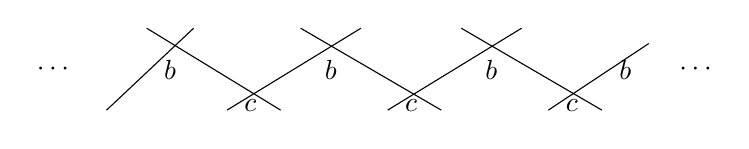
\begin{tikzpicture}[x=0.85cm,y=0.65cm]
\node at (-0.8,0) {$\cdots$};\node at (8.8,0) {$\cdots$};
\draw (0,-.8)--(1.3,.8);\draw (.6,.8)--(2.6,-.8);
\draw (1.8,-.8)--(3.8,.8);\draw (2.9,.8)--(5,-.8);
\draw (4.2,-.8)--(6.2,.8);\draw (5.3,.8)--(7.4,-.8);
\draw (6.6,-.8)--(8.1,.5);
\node[below] at (.95,.37) {$b$};\node[below] at (3.35,.37) {$b$};\node[below] at (5.75,.37) {$b$};\node[below] at (7.75,.37) {$b$};
\node[below] at (2.15,-.4) {$c$};\node[below] at (4.55,-.4) {$c$};\node[below] at (6.95,-.4) {$c$};
\end{tikzpicture}
\end{center}
（注意：这里的\Term{principal-bundle}{主纤维丛}是在\Term{etale-topology}{平展拓扑}意义下的。）又有\Term{homomorphism}{同态}
\[
\varphi:\mathbf Z\longrightarrow\operatorname{GL}(2,\mathbf Z),\qquad
\varphi(n)=\begin{pmatrix}1&n\\0&1\end{pmatrix},
\]
这使我们可由 $P$ 上的\Term{trivial}{平凡}\Term{torus}{环面} $\mathbf G_m^2$ 及由 $\varphi$ \Term{derive}{导出}的\Term{descent-datum}{下降数据}，构造 $S$ 上相对\Term{dimension}{维数}为 $2$ 的\Term{torus}{环面} $T$。（注意：\Term{projection}{投影} $P\to S$ 是\Term{etale-topology}{平展拓扑}的\Term{covering-morphism}{覆盖态射}，因而也是 $(\mathrm{Sch})$ 的\Term{canonical-topology}{典范拓扑}的\Term{covering-morphism}{覆盖态射}；而所考察的\Term{descent-datum}{下降数据}必\Term{effective}{有效}，因为 $\mathbf G_{m,P}^2$ 在 $P$ 上\Term{affine}{仿射}。）不难证明，$T$ 在 $a$ 的任何\Term{neighborhood}{邻域}中都不\Term{isotrivial}{等平凡}\footnote[5]{编者注：见下文 7.3。}（但它在 $S-\{a\}$ 上\Term{trivial}{平凡}）。

取 $S$ 为有两个\Term{irreducible-component}{不可约分支} $S_1,S_2$、且它们相交于两点 $a',a''$ 的\Term{curve}{曲线}，就得到此构造的一个变体。这使我们能构造 $S$ 上群为 $\mathbf Z_S$ 的\Term{connected}{连通}且\Term{locally-trivial}{局部平凡}的\Term{principal-homogeneous-bundle}{主齐性纤维丛} $P$，从而得到一个\Term{locally-trivial}{局部平凡}但不\Term{isotrivial}{等平凡}的\Term{adjunction}{伴随}\Term{torus}{环面} $T$。
\SGAsection{2}{结构的无穷小变化}
先回顾下述结果\footnote[6]{编者注：加入此“回顾”，供后文引用。}（$S$ \Term{locally-noetherian}{局部诺特}时见 SGA 1，第 I 讲 8.3；一般情形见 EGA IV$_4$，18.1.2）。
\SourcePage{66}
\begin{SGAresult}{回顾}{2.0}
设 $S$ 为\Term{prescheme}{预概形}，$S_0$ 为具有相同\Term{underlying-set}{底集}的\Term{subprescheme}{子预概形}。则\Term{functor}{函子}
\[
X\longmapsto X_0=X\times_S S_0
\]
给出 $S$ 上\Term{etale}{平展}\Term{prescheme}{预概形}\Term{category}{范畴}与 $S_0$ 上相应\Term{category}{范畴}之间的\Term{equivalence}{等价}。
\end{SGAresult}
\begin{SGAresult}{命题}{2.1}
设 $S$ 为\Term{prescheme}{预概形}，$S_0$ 为具有相同\Term{underlying-set}{底集}的\Term{subprescheme}{子预概形}（即由一个\Term{nilideal}{零理想} $\mathscr I$ 定义）。则\Term{functor}{函子}
\[
H\longmapsto H_0=H\times_S S_0
\]
从 $S$ 上\Term{multiplicative-type}{乘法型群}\Term{prescheme}{预概形}\Term{category}{范畴}到 $S_0$ 上相应\Term{category}{范畴}是\Term{fully-faithful}{全忠实}的。

此外，它诱导 $S$ 上\Term{quasi-isotrivial}{拟等平凡}\Term{multiplicative-type}{乘法型群}\Term{category}{范畴}与 $S_0$ 上相应\Term{category}{范畴}之间的\Term{equivalence}{等价}。
\end{SGAresult}
\begin{proof}
先证\Term{fully-faithful}{全忠实性}，即对 $S$ 上\Term{multiplicative-type}{乘法型群} $H,G$，映射
\[
\operatorname{Hom}_{S\text{-gr.}}(H,G)\longrightarrow
\operatorname{Hom}_{S_0\text{-gr.}}(H_0,G_0)
\]
为\Term{bijective}{双射}。问题在 $S$ 上是\Term{local-scheme}{局部}的，可假定 $S$ \Term{affine}{仿射}。于是存在\Term{faithfully-flat}{忠实平坦}\Term{quasi-compact}{拟紧}\Term{morphism}{态射} $S'\to S$ \Term{split}{分裂} $H,G$。令 $S''=S'\times_S S'$，用 $H',G'$（分别 $H'',G''$）\Term{representation}{表示} $H,G$ 经\Term{base-change}{基变换} $S'\to S$（分别 $S''\to S$）所得的群；同样定义 $S'_0,S''_0$，其中后者也\Term{isomorphism}{同构}于 $S'_0\times_{S_0}S'_0$。于是有各行\Term{exact}{正合}的\Term{commutative-diagram}{交换图}：
\[
\begin{tikzcd}[column sep=small]
\operatorname{Hom}_{S\text{-gr.}}(H,G)\arrow[r]\arrow[d,"u"] &
\operatorname{Hom}_{S'\text{-gr.}}(H',G')\arrow[r,shift left=.45ex]\arrow[r,shift right=.45ex]\arrow[d,"u'"] &
\operatorname{Hom}_{S''\text{-gr.}}(H'',G'')\arrow[d,"u''"]\\
\operatorname{Hom}_{S_0\text{-gr.}}(H_0,G_0)\arrow[r]&
\operatorname{Hom}_{S'_0\text{-gr.}}(H'_0,G'_0)\arrow[r,shift left=.45ex]\arrow[r,shift right=.45ex]&
\operatorname{Hom}_{S''_0\text{-gr.}}(H''_0,G''_0).
\end{tikzcd}
\]
故为证 $u$ \Term{bijective}{双射}，只需证 $u',u''$ \Term{bijective}{双射}。这将我们归结到 $H,G$ \Term{diagonalizable}{可对角化}，因而分别形如 $D_S(M),D_S(N)$ 的情形，其中 $M,N$ 为通常意义的\Term{commutative-group}{交换群}。于是同样有 $H_0=D_{S_0}(M)$，$G_0=D_{S_0}(N)$。此时有\Term{commutative-diagram}{交换图}\footnote[7]{编者注：已将右侧各项中的 $M,N$ 对调，以修正原文。}
\[
\begin{tikzcd}
\operatorname{Hom}_{S\text{-gr.}}(N_S,M_S)\arrow[r,"\sim"]\arrow[d]&
\operatorname{Hom}_{S\text{-gr.}}(D_S(M),D_S(N))\arrow[d]\\
\operatorname{Hom}_{S_0\text{-gr.}}(N_{S_0},M_{S_0})\arrow[r,"\sim"]&
\operatorname{Hom}_{S_0\text{-gr.}}(D_{S_0}(M),D_{S_0}(N)),
\end{tikzcd}
\]
\SourcePage{67}
由第 VIII 讲 1.4，水平\Term{arrow}{箭头}为\Term{isomorphism}{同构}。因而归结到证明\Term{homomorphism}{同态}
\[
\operatorname{Hom}_{S\text{-gr.}}(N_S,M_S)\longrightarrow
\operatorname{Hom}_{S_0\text{-gr.}}(N_{S_0},M_{S_0})\tag{x}
\]
为\Term{bijective}{双射}，即证明 $M_S\mapsto M_{S_0}$ 这个从 $S$ 上常值\Term{commutative-group}{交换群}\Term{prescheme}{预概形}到 $S_0$ 上相应\Term{prescheme}{预概形}的\Term{functor}{函子}\Term{fully-faithful}{全忠实}。而 (x) 也可等同于自然映射
\[
\operatorname{Hom}_{\mathrm{gr.}}(N,\Gamma(M_S))\longrightarrow
\operatorname{Hom}_{\mathrm{gr.}}(N,\Gamma(M_{S_0})),
\]
它由 $\Gamma(M_S)\to\Gamma(M_{S_0})$ \Term{derive}{导出}。后一个映射显然为\Term{bijective}{双射}（因为 $\Gamma(M_S)$ 是 $S$ 到 $M$ 的\Term{locally-constant-map}{局部常值映射}的\Term{set}{集合}，只依赖于 $S$ 的\Term{underlying-topological-space}{底拓扑空间}），由此得到所需结论。

要证 2.1 的第二个断言，只须证明 $S_0$ 上每个\Term{quasi-isotrivial}{拟等平凡}\Term{multiplicative-type}{乘法型群} $H_0$ 都来自 $S$ 上一个\Term{quasi-isotrivial}{拟等平凡}\Term{multiplicative-type}{乘法型群} $H$。为此，取\Term{split}{分裂} $H_0$ 的\Term{etale}{平展}\Term{surjective}{满射} $S'_0\to S_0$。

由 2.0，存在\Term{etale}{平展}\Term{morphism}{态射} $S'\to S$ 及 $S_0$ \Term{isomorphism}{同构} $S'\times_S S_0\simeq S'_0$，故可假定 $S'_0$ 由 $S'$ \Term{reduced}{约化}而来。由于 $H'_0$ \Term{diagonalizable}{可对角化}，立即看出它\Term{isomorphism}{同构}于 $S'$ 上某个\Term{diagonalizable}{可对角化}群 $H'$ 经\Term{base-change}{基变换} $S'_0\to S'$ 所得的群。（注意：若 $H'_0=D_{S'_0}(M)$，可取 $H'=D_{S'}(M)$。）照例令 $S''=S'\times_S S'$，$S'''=S'\times_S S'\times_S S'$；同样定义 $S''_0,S'''_0$，它们由前者经\Term{base-change}{基变换} $S_0\to S$ 得到，也\Term{isomorphism}{同构}于 $S'_0$ 在 $S_0$ 上的\Term{fiber}{纤维}平方和\Term{fiber}{纤维}立方。将已经证明的\Term{fully-faithful}{全忠实性}用于 $(S'',S''_0)$ 及 $(S''',S'''_0)$，可见 $H'_0$ 关于 $S'_0\to S_0$ 的自然\Term{descent-datum}{下降数据}（见第 IV 讲 2.1），来自 $H'$ 关于 $S'\to S$ 的一个唯一确定的\Term{descent-datum}{下降数据}。此\Term{descent-datum}{下降数据}\Term{effective}{有效}，因为 $H'$ 在 $S'$ 上\Term{affine}{仿射}（SGA 1，第 VIII 讲 2.1），故存在 $S$ 群 $H$，使 $H\times_S S'=H'=D_{S'}(M)$；所以 $H$ 是\Term{quasi-isotrivial}{拟等平凡}\Term{multiplicative-type}{乘法型群}。

再对 $(S',S'_0)$ 应用\Term{fully-faithful}{全忠实性}，容易验证 $H'_0$ 与 $H'\times_{S'}S'_0$ 之间给定的\Term{isomorphism}{同构}来自 $H_0$ 与 $H\times_S S_0$ 之间的\Term{isomorphism}{同构}。（这类结果更正式的论述见 Giraud 正在准备的关于\Term{descent}{下降}理论的文章。\footnote{见 J. Giraud，\emph{Méthode de la descente}，Bull. Soc. Math. France，Mémoire 2，(1964)。}）
\end{proof}
\begin{SGAresult}{推论}{2.2}
设 $H$ 为\Term{multiplicative-type}{乘法型} $S$ 群，$H_0=H\times_S S_0$。则 $H$ 为\Term{quasi-isotrivial}{拟等平凡}（分别\Term{locally-isotrivial}{局部等平凡}、\Term{isotrivial}{等平凡}、\Term{locally-trivial}{局部平凡}、\Term{trivial}{平凡}）的充要条件是 $H_0$ 具有相应性质。
\end{SGAresult}
\begin{proof}
必要性显然。\Term{quasi-isotrivial}{拟等平凡}情形的充分性已经证明，因为由\Term{fully-faithful}{全忠实性}，只须知道每个 $S_0$ 上\Term{quasi-isotrivial}{拟等平凡}群均可\Term{lifting}{提升}为 $S$ 上\Term{quasi-isotrivial}{拟等平凡}群。同一论证也适用于“\Term{trivial}{平凡}”。对“\Term{isotrivial}{等平凡}”情形，重复证明 2.1 第二个断言的论证，但取 $S'_0\to S_0$ 为\Term{finite-etale}{有限平展}\Term{surjective}{满射}。“\Term{locally-isotrivial}{局部等平凡}”和“\Term{locally-trivial}{局部平凡}”情形立即由“\Term{isotrivial}{等平凡}”和“\Term{trivial}{平凡}”情形得出。
\end{proof}
当 $\mathscr I$ \Term{nilpotent}{幂零}时，可以稍微推广 2.2，不预先假定 $H$ 为\Term{multiplicative-type}{乘法型群}：\footnote[8]{编者注：提醒读者，2.3 用于证明第 IX 讲\Term{theorem}{定理} 3.6 bis。}
\SourcePage{68}
\begin{SGAresult}{推论}{2.3}
假定定义 $S_0$ 的\Term{ideal}{理想} $\mathscr I$ \Term{locally-nilpotent}{局部幂零}。设 $H$ 为 $S$ 上的\Term{group-prescheme}{群预概形}，在 $S$ 上\Term{flat}{平坦}，且 $H_0=H\times_S S_0$。则 $H$ 为\Term{quasi-isotrivial}{拟等平凡}\Term{multiplicative-type}{乘法型群}的充要条件是 $H_0$ 具有此性质。
\end{SGAresult}
\begin{proof}
假定 $H_0$ 为\Term{quasi-isotrivial}{拟等平凡}\Term{multiplicative-type}{乘法型群}，来证 $H$ 亦然。问题在\Term{etale-topology}{平展拓扑}下是\Term{local-scheme}{局部}的，而\Term{functor}{函子} $S'\mapsto S'\times_S S_0$ 给出 $S$ 上\Term{etale}{平展}\Term{prescheme}{预概形}\Term{category}{范畴}与 $S_0$ 上\Term{etale}{平展}\Term{prescheme}{预概形}\Term{category}{范畴}的\Term{equivalence}{等价}（见 2.0），故立即归结到 $H_0$ \Term{diagonalizable}{可对角化}，因而\Term{isomorphism}{同构}于某个 $D_{S_0}(M)$ 的情形。令 $G=D_S(M)$，则有\Term{isomorphism}{同构} $u_0:H_0\xrightarrow{\sim}G_0$。我断言，它来自唯一的\Term{homomorphism}{同态} $u:H\to G$；由于 $u_0$ 为\Term{isomorphism}{同构}，$u$ 也为\Term{isomorphism}{同构}（因 $H,G$ 在 $S$ 上\Term{flat}{平坦}，且 $\mathscr I$ \Term{locally-nilpotent}{局部幂零}\footnote[9]{编者注：由于 $u_0$ 为\Term{isomorphism}{同构}，只须证明，对每个 $h\in H$，\Term{morphism}{态射} $\phi:\mathscr O_{G,u(h)}\to\mathscr O_{H,h}$ 为\Term{bijective}{双射}。\Term{module}{模} $I=\mathscr I_s$ \Term{reduced}{约化}后它为\Term{bijective}{双射}（其中 $s$ 为 $h$ 在 $S$ 中的像），所以其\Term{cokernel}{余核} $C$ 满足 $C=IC$，因 $I$ \Term{nilpotent}{幂零}而有 $C=0$。于是，由于 $\mathscr O_{H,h}$ 在 $\mathscr O_{S,s}$ 上\Term{flat}{平坦}，$\phi$ 的核 $K$ 也满足 $K=IK$，故 $K=0$。}），这将证明 2.3。又有（见第 VIII 讲 1 (xxx)）
\[
\operatorname{Hom}_{S\text{-gr.}}(H,G)\simeq
\operatorname{Hom}_{S\text{-gr.}}(M_S,\underline{\operatorname{Hom}}_{S\text{-gr.}}(H,\mathbf G_{m,S})),
\]
其右端也等同于
\[
\operatorname{Hom}_{\mathrm{gr.}}(M,\operatorname{Hom}_{S\text{-gr.}}(H,\mathbf G_{m,S})).
\]
故\Term{homomorphism}{同态}
\[
\operatorname{Hom}_{S\text{-gr.}}(H,G)\longrightarrow\operatorname{Hom}_{S_0\text{-gr.}}(H_0,G_0)\tag{x}
\]
\Term{isomorphism}{同构}于由\Term{restriction}{限制}\Term{homomorphism}{同态}
\[
\operatorname{Hom}_{S\text{-gr.}}(H,\mathbf G_{m,S})\longrightarrow
\operatorname{Hom}_{S_0\text{-gr.}}(H_0,\mathbf G_{m,S_0})\tag{xx}
\]
\Term{derive}{导出}的\Term{homomorphism}{同态}
\[
\operatorname{Hom}_{\mathrm{gr.}}(M,\operatorname{Hom}_{S\text{-gr.}}(H,\mathbf G_{m,S}))
\longrightarrow
\operatorname{Hom}_{\mathrm{gr.}}(M,\operatorname{Hom}_{S_0\text{-gr.}}(H_0,\mathbf G_{m,S_0})).
\]
因此为证 (x) \Term{bijective}{双射}，只须证 (xx) \Term{bijective}{双射}。问题在 $S$ 上是\Term{local-scheme}{局部}的，故可假定 $S$ \Term{affine}{仿射}。由于 $\mathbf G_{m,S}$ 在 $S$ 上交换且\Term{smooth}{光滑}，可应用第 IX 讲 3.6，证明完毕。
\end{proof}
\begin{SGAresult}{推论}{2.4}
设 $A$ 为\Term{residue-field}{剩余域}为 $k$ 的\Term{local-artinian-ring}{局部阿廷环}，$S=\operatorname{Spec}(A)$，$S_0=\operatorname{Spec}(k)$。

(i)\footnote[10]{编者注：重写此陈述，仅保留非\Term{trivial}{平凡}的蕴涵，以突出该蕴涵。} 设 $H$ 为\Term{flat}{平坦}且\Term{locally-finite-type}{局部有限型}的 $S$ \Term{group-prescheme}{群预概形}，使 $H_0=H\times_S S_0$ 为\Term{multiplicative-type}{乘法型群}。则 $H$ 为\Term{finite-type}{有限型}且\Term{isotrivial}{等平凡}的\Term{multiplicative-type}{乘法型群}。特别地，每个\Term{finite-type}{有限型}\Term{multiplicative-type}{乘法型} $S$ \Term{group-prescheme}{群预概形} $H$ 都\Term{isotrivial}{等平凡}。

(ii) \Term{functor}{函子} $H\mapsto H_0$ 给出 $A$ 上\Term{finite-type}{有限型}\Term{multiplicative-type}{乘法型群}\Term{category}{范畴}与 $k$ 上相应\Term{category}{范畴}之间的\Term{equivalence}{等价}。
\end{SGAresult}
\SourcePage{69}
\begin{proof}
设 $H$ 如 (i) 中所述。则 $H_0$ 为\Term{locally-finite-type}{局部有限型}的\Term{multiplicative-type}{乘法型群}，故为\Term{finite-type}{有限型}，从而由 1.4 为\Term{isotrivial}{等平凡}。因此由 2.3、2.2，$H$ 为\Term{multiplicative-type}{乘法型群}（因而为\Term{finite-type}{有限型}）且\Term{isotrivial}{等平凡}。断言 (ii) 遂由 2.1 得出。
\end{proof}
\begin{SGAresult}{推论}{2.5}
设 $S'\to S$ 为\Term{faithfully-flat}{忠实平坦}\Term{radicial}{根性}\Term{morphism}{态射}。

(i) \Term{functor}{函子} $H\mapsto H'=H\times_S S'$ 从 $S$ 上\Term{multiplicative-type}{乘法型群}\Term{category}{范畴}到 $S'$ 上相应\Term{category}{范畴}是\Term{fully-faithful}{全忠实}的。

此外，它在由\Term{quasi-isotrivial}{拟等平凡}\Term{multiplicative-type}{乘法型群}组成的子\Term{category}{范畴}之间诱导\Term{equivalence}{等价}。

(ii) 若 $H$ 为\Term{multiplicative-type}{乘法型群}，则它为\Term{quasi-isotrivial}{拟等平凡}（分别\Term{locally-isotrivial}{局部等平凡}、\Term{isotrivial}{等平凡}、\Term{locally-trivial}{局部平凡}、\Term{trivial}{平凡}）的充要条件是 $H'$ 具有相应性质。
\end{SGAresult}
\begin{proof}
令 $S''=S'\times_S S'$，$S'''=S'\times_S S'\times_S S'$。$S'\to S$ \Term{radicial}{根性}的假设意味着对角\Term{immersion}{浸入} $S'\to S''$ 及 $S'\to S'''$ 均\Term{surjective}{满射}，因此由其中任一\Term{immersion}{浸入}所作的\Term{base-change}{基变换}都可应用 2.1、2.2。又因 $S'\to S$ 为\Term{faithfully-flat}{忠实平坦}\Term{quasi-compact}{拟紧}\Term{morphism}{态射}\footnote[11]{编者注：须详细说明这一点……}，所以它对\Term{prescheme}{预概形}上的\Term{multiplicative-type}{乘法型群}\Term{fibered-category}{纤维范畴}是\Term{effective-descent}{有效下降}\Term{morphism}{态射}；计及此点，我们的断言\Term{form}{形式}地由 2.1、2.2 得出（完\Term{integral-morphism}{整}的论证见前引 Giraud 的文章）。
\end{proof}
\SGAsection{3}{结构的有限变化：完备基环}
\begin{SGAresult}{\Term{lemma}{引理}}{3.1}
设 $A$ 为\Term{noetherian-ring}{诺特环}，配有\Term{ideal}{理想} $I$，且 $A$ 关于 $I$ 进\Term{topology}{拓扑}\Term{separated}{分离}且\Term{complete}{完备}；令 $S=\operatorname{Spec}(A)$，$S_0=\operatorname{Spec}(A/I)$。设 $G,H$ 为两个 $S$ \Term{group-scheme}{群概形}，其中 $G$ 为\Term{isotrivial}{等平凡}\Term{multiplicative-type}{乘法型群}，$H$ 在 $S$ 上\Term{affine}{仿射}，在 $H_0=H\times_S S_0$ 各点处对 $S$ \Term{flat}{平坦}，且 $H_0$ 为\Term{quasi-isotrivial}{拟等平凡}\Term{multiplicative-type}{乘法型群}。则自然映射
\[
\operatorname{Hom}_{S\text{-gr.}}(G,H)\longrightarrow
\operatorname{Hom}_{S_0\text{-gr.}}(G_0,H_0)
\]
为\Term{bijective}{双射}。
\end{SGAresult}
\begin{proof}
对每个\Term{integral-morphism}{整}数 $n\geq0$，令 $S_n=\operatorname{Spec}(A/I^{n+1})$，并令 $G_n,H_n$ 为 $G,H$ 经\Term{base-change}{基变换} $S_n\to S$ 所得的群。由于 $G/S$ 为\Term{isotrivial}{等平凡}\Term{multiplicative-type}{乘法型群}且 $H$ 在 $S$ 上\Term{affine}{仿射}，第 IX 讲 7.1 表明自然\Term{homomorphism}{同态}
\[
\operatorname{Hom}_{S\text{-gr.}}(G,H)\longrightarrow
\varprojlim_n\operatorname{Hom}_{S_n\text{-gr.}}(G_n,H_n)
\]
为\Term{bijective}{双射}。另一方面，由 2.3，各 $H_n$ 为\Term{quasi-isotrivial}{拟等平凡}\Term{multiplicative-type}{乘法型群}，而由 2.1，\Term{projective-system}{投射系} $(\operatorname{Hom}_{S_n\text{-gr.}}(G_n,H_n))_n$ 的过渡\Term{homomorphism}{同态}为\Term{isomorphism}{同构}，立即得出 3.1。
\end{proof}
\begin{SGAresult}{\Term{theorem}{定理}}{3.2}
设 $A$ 为\Term{noetherian-ring}{诺特环}，配有\Term{ideal}{理想} $I$，且 $A$ 关于 $I$ 进\Term{topology}{拓扑}\Term{separated}{分离}且\Term{complete}{完备}；令 $S=\operatorname{Spec}(A)$，$S_0=\operatorname{Spec}(A/I)$。则：
\SourcePage{70}
(i) \Term{functor}{函子}
\[
H\longmapsto H_0=H\times_S S_0
\]
给出 $S$ 上\Term{isotrivial}{等平凡}\Term{multiplicative-type}{乘法型群}\Term{category}{范畴}与 $S_0$ 上相应\Term{category}{范畴}之间的\Term{equivalence}{等价}。

(ii) 设 $H$ 为\Term{finite-type}{有限型}\Term{multiplicative-type}{乘法型} $S$ 群；则 $H$ \Term{isotrivial}{等平凡}的充要条件是 $H_0$ \Term{isotrivial}{等平凡}。
\end{SGAresult}
\begin{proof}
对 (i)，可以重复 2.1 的证明，也可以利用 1.2；两种方法都利用\Term{functor}{函子}
\[
S'\longmapsto S'_0=S'\times_S S_0
\]
给出 $S$ 上\Term{finite-etale}{有限平展}\Term{scheme}{概形}\Term{category}{范畴}与 $S_0$ 上\Term{finite-etale}{有限平展}\Term{scheme}{概形}\Term{category}{范畴}之间的\Term{equivalence}{等价}（SGA 1，第 I 讲 8.4）。这也\Term{representable}{可表}述为（归结到 $S$ \Term{connected}{连通}，即 $S_0$ \Term{connected}{连通}的情形），选取 $S_0$ 的一个\Term{geometric-point}{几何点} $\xi$ 后，\Term{canonical}{典范}\Term{homomorphism}{同态}
\[
\pi_1(S_0,\xi)\longrightarrow\pi_1(S,\xi)
\]
为\Term{isomorphism}{同构}。

证明 (ii)，即若 $H_0$ \Term{isotrivial}{等平凡}，则 $H$ \Term{isotrivial}{等平凡}。由 (i)，存在 $S$ 上\Term{isotrivial}{等平凡}\Term{multiplicative-type}{乘法型群} $G$ 及 $S_0$ \Term{isomorphism}{同构}
\[
u_0:G_0\xrightarrow{\sim}H_0.
\]
由于 $H$ 为\Term{finite-type}{有限型}，$H_0,G_0$ 亦然；故由第 IX 讲 2.1 b)，$G$ 在 $S$ 每一点的型为\Term{finitely-generated}{有限生成}\Term{abelian-group}{阿贝尔群}，所以 $G$ 在 $S$ 上\Term{finite-type}{有限型}。\footnote[12]{编者注：下文对原文作了详细展开。} 另一方面，由 3.1，$u_0$ 来自 $S$ 群\Term{homomorphism}{同态}
\[
u:G\longrightarrow H.
\]
最后，$G,H$ 是 $S$ 上的\Term{finite-type}{有限型}\Term{multiplicative-type}{乘法型群}，而 $u_0$ 为\Term{isomorphism}{同构}，故由第 IX 讲 2.9，$u$ 为\Term{isomorphism}{同构}（这里计及 $S$ 中 $S_0$ 的每个\Term{neighborhood}{邻域}都等于 $S$）。
\end{proof}
\begin{SGAresult}{推论}{3.3}
设 $A$ 为\Term{residue-field}{剩余域}为 $k$ 的\Term{complete}{完备}\Term{local-noetherian-ring}{局部诺特环}。

(i) $A$ 上每个\Term{finite-type}{有限型}\Term{multiplicative-type}{乘法型群}均\Term{isotrivial}{等平凡}。

(ii) \Term{functor}{函子} $H\mapsto H\otimes_A k=H_0$ 给出 $A$ 上\Term{finite-type}{有限型}\Term{multiplicative-type}{乘法型群}\Term{category}{范畴}与 $k$ 上相应\Term{category}{范畴}之间的\Term{equivalence}{等价}。
\end{SGAresult}
\begin{proof}
首先，(i) 由 3.2 (ii) 及 1.4 得出；(ii) 遂由 3.2 (i) 得出，只需计及 $H$ 为\Term{finite-type}{有限型}当且仅当 $H_0$ 为\Term{finite-type}{有限型}（见 3.2 (ii) 的证明）。\footnotemark[12]
\end{proof}
\textbf{注记 3.3.1。}注意，由 1.4，3.3 用 $k$ 的一个\Term{algebraic-closure}{代数闭包} $\Omega$ 的\Term{topological-galois-group}{拓扑 Galois 群}给出了 $A$ 上\Term{finite-type}{有限型}\Term{multiplicative-type}{乘法型群}的完\Term{integral-morphism}{整}分类。
\SourcePage{71}
\textbf{注记 3.4。}在 3.2 的假设下（即 $A$ 为\Term{noetherian-ring}{诺特环}，关于 $I$ 进\Term{topology}{拓扑}\Term{separated}{分离}且\Term{complete}{完备}，而对 $A/I$ 无其他假设），由第 5 节将知，\Term{functor}{函子} $H\mapsto H_0$ 从 $S$ 上\Term{finite-type}{有限型}\Term{multiplicative-type}{乘法型群}\Term{category}{范畴}到 $S_0$ 上相应\Term{category}{范畴}仍为\Term{fully-faithful}{全忠实}的（无需\Term{isotrivial}{等平凡性}假设）。\footnote[13]{编者注：须明确此引用，或在第 5 节补入一个推论……}

但它一般并非\Term{essentially-surjective}{本质满}的；事实上，可能存在\Term{finite-type}{有限型}\Term{multiplicative-type}{乘法型} $S_0$ 群 $H_0$，甚至可令其\Term{locally-trivial}{局部平凡}（但不\Term{isotrivial}{等平凡}），使它不是 $S$ 上某个\Term{multiplicative-type}{乘法型群} $H$ 的\Term{reduced}{约化}。

为说明这一点，重取 1.6 中非\Term{normal}{正规}\Term{curve}{曲线}上非\Term{isotrivial}{等平凡}\Term{multiplicative-type}{乘法型群}的任一例子。显然可以取该\Term{curve}{曲线}为\Term{affine}{仿射}的，记为 $S_0$，并假定其\Term{embedding}{嵌入}二维\Term{affine}{仿射}\Term{space}{空间}，从而由 $k[X,Y]$ 中的\Term{ideal}{理想} $J$ 定义。取 $A$ 为此环关于 $J$ 预进\Term{topology}{拓扑}的\Term{completion}{完备化}；于是 $A$ 是一个二维\Term{regular-ring}{正则环}，因而\Term{normal}{正规}。将在 5.16 看到，这意味着 $S=\operatorname{Spec}(A)$ 上每个\Term{finite-type}{有限型}\Term{multiplicative-type}{乘法型群}均\Term{isotrivial}{等平凡}；所以\Term{finite-type}{有限型}但不\Term{isotrivial}{等平凡}的 $H_0$ 不来自 $S$ 上的\Term{multiplicative-type}{乘法型群} $H$（因为 $H$ 必为\Term{finite-type}{有限型}，从而\Term{isotrivial}{等平凡}）。
\begin{SGAresult}{\Term{lemma}{引理}}{3.5}
设 $S$ 为\Term{prescheme}{预概形}，$u:G\to H$ 为\Term{locally-finite-presentation}{局部有限表示}且在 $S$ 上\Term{flat}{平坦}的 $S$ \Term{group-prescheme}{群预概形}的\Term{homomorphism}{同态}；令 $U$ 为那些使\Term{fiber}{纤维}上诱导的\Term{homomorphism}{同态} $u_s:G_s\to H_s$ \Term{flat}{平坦}（分别\Term{smooth}{光滑}、\Term{unramified}{非分歧}、\Term{etale}{平展}、\Term{quasi-finite}{拟有限}）的 $s\in S$ 所成的\Term{set}{集合}。\footnote{这类结果更系统的展开也见第 VI$_B$ 讲 2.5。}

则 $U$ 为\Term{open-subset}{开集}，且\Term{restriction}{限制} $u|_U:G|_U\to H|_U$ 为\Term{flat}{平坦}（分别\Term{smooth}{光滑}、\Term{unramified}{非分歧}、\Term{etale}{平展}、\Term{quasi-finite}{拟有限}）\Term{morphism}{态射}。
\end{SGAresult}
\begin{proof}
令 $V$ 为 $u$ \Term{flat}{平坦}（分别具有上述性质）的点集。已知 $V$ 为\Term{open-subset}{开集}（\Term{locally-noetherian}{局部诺特}情形见 SGA 1，第 I 至 IV 讲，一般情形见 EGA IV\footnote[14]{编者注：须明确这些引用：由于 $G,H$ \Term{locally-finite-presentation}{局部有限表示}，$u$ 亦\Term{locally-finite-presentation}{局部有限表示}（IV$_1$，1.4.3 (v)）；然后对\Term{flat}{平坦}及\Term{quasi-finite}{拟有限}应用 IV$_3$，11.3.10、13.1.4，对\Term{unramified}{非分歧}、\Term{smooth}{光滑}及\Term{etale}{平展}应用 IV$_4$，17.4.1、17.5.1、17.6.1；与第 VI$_B$ 讲 2.5 比较。}），且对位于 $s\in S$ 上方的 $x\in G$，有 $x\in V$ 当且仅当 $u_s:G_s\to H_s$ 在 $x$ 处\Term{flat}{平坦}（分别具有相应性质）（引用同前；在\Term{flat}{平坦}、\Term{smooth}{光滑}、\Term{etale}{平展}的情形，此处用到 $G,H$ 在 $S$ 上\Term{flat}{平坦}）。由于 $u_s$ 为\Term{locally-algebraic-group}{局部代数群}的\Term{homomorphism}{同态}，这也意味着 $u_s$ 处处\Term{flat}{平坦}（分别具有相应性质）（第 VI$_B$ 讲 1.3），即 $s\in U$。故 $U$ 是\Term{open-subset}{开集} $V$ 在 $G$ 的\Term{unit-section}{单位截面}下的\Term{inverse-image}{逆像}，因而开，且 $V=G|_U$；于是 $G|_U\to H|_U$ \Term{flat}{平坦}（分别具有相应性质），证明完毕。（注意：在“\Term{unramified}{非分歧}”或“\Term{quasi-finite}{拟有限}”情形中，无须假定 $G,H$ \Term{flat}{平坦}。）
\end{proof}
\begin{SGAresult}{\Term{lemma}{引理}}{3.6}
设 $H$ 为域 $k$ 上的交换\Term{algebraic-group}{代数群}，有一个\Term{multiplicative-type}{乘法型}\Term{open-subgroup}{开子群} $G$。则 $H$ 的\Term{subscheme}{子概形}族 ${}_nH$（$n>0$）在 $H$ 中\Term{schematically-dense}{概形稠密}；特别地，若对一切 $n>0$ 均有 ${}_nH={}_nG$，则 $H=G$。
\end{SGAresult}
\SourcePage{72}
\begin{proof}
这里 ${}_nH$ \Term{representation}{表示} $n\cdot\operatorname{id}_H$ 的核。\footnote[15]{编者注：加入了接下来的一句。} 令 $\bar k$ 为 $k$ 的一个\Term{algebraic-closure}{代数闭包}；只须证明族 $({}_nH_{\bar k})_{n>0}$ 在 $H_{\bar k}$ 中\Term{schematically-dense}{概形稠密}，因为这样 $({}_nH)_{n>0}$ 在 $H$ 中也\Term{schematically-dense}{概形稠密}（见第 IX 讲 4.5）。所以可假定 $k$ \Term{algebraically-closed}{代数闭}，从而 $G$ 形如 $D_k(M)$，其中 $M$ 为通常意义的\Term{finitely-generated}{有限生成}\Term{commutative-group}{交换群}。令 $M_0=M/\operatorname{Torsion}(M)$，则 $T=D_k(M_0)$ 是包含于 $G$ 的最大\Term{torus}{环面}，而 $H/T$ \Term{finite}{有限}，故 $H(k)/T(k)$ 被某个\Term{integral-morphism}{整}数 $\nu>0$ \Term{annihilate}{零化}。可取\Term{finite}{有限}多个元素 $g_i\in H(k)$，使
\[
H=\coprod_i g_i\cdot G,
\]
并有 $g_i^\nu\in T(k)$。由于 $k$ \Term{algebraically-closed}{代数闭}，$\nu\cdot\operatorname{id}_T$ 在 $T(k)\simeq k^{*d}$ 上\Term{surjective}{满射}，因此将 $g_i$ 换成 $g_it_i^{-1}$（其中 $t_i\in T(k)$ 满足 $t_i^\nu=g_i^\nu$）后，可假定 $g_i^\nu=1$。若 $n$ 是 $\nu$ 的倍数，则有
\[
{}_nH\supseteq g_i\cdot{}_nG.
\]
由第 IX 讲 4.7，族 ${}_nG$（$n>0$ 变化）在 $G$ 中\Term{schematically-dense}{概形稠密}，故得到 3.6 的结论。
\end{proof}
\begin{SGAresult}{\Term{theorem}{定理}}{3.7}
设 $A$ 为\Term{noetherian-ring}{诺特环}，配有\Term{ideal}{理想} $I$，且 $A$ 关于 $I$ 进\Term{topology}{拓扑}\Term{separated}{分离}且\Term{complete}{完备}；令 $S=\operatorname{Spec}(A)$，$S_0=\operatorname{Spec}(A/I)$。设 $H$ 为\Term{finite-type}{有限型}\Term{affine}{仿射} $S$ \Term{group-scheme}{群概形}，在 $H_0$ 各点处对 $S$ \Term{flat}{平坦}，且 $H_0=H\times_S S_0$ 为\Term{isotrivial}{等平凡}\Term{multiplicative-type}{乘法型群}。

则 $H$ 有一个既开又闭的\Term{subgroup}{子群} $G$，它是\Term{isotrivial}{等平凡}\Term{multiplicative-type}{乘法型群}（且为\Term{finite-type}{有限型}），并满足 $G_0=H_0$。
\end{SGAresult}
\begin{proof}
由 3.2 (i)，存在 $S$ 上\Term{isotrivial}{等平凡}\Term{multiplicative-type}{乘法型群} $G$ 及\Term{isomorphism}{同构}
\[
u_0:G_0\xrightarrow{\sim}H_0.
\]
由 3.1，$u_0$ 来自唯一的 $S$ 群\Term{homomorphism}{同态}
\[
u:G\longrightarrow H.
\]
利用第 IX 讲 6.6，可知 $u$ 为\Term{monomorphism}{单态射}（因为若 $U$ 为使 $u_s:G_s\to H_s$ 为\Term{monomorphism}{单态射}的 $s\in S$ 所成的\Term{set}{集合}，则 $U$ 是 $S_0$ 的一个\Term{open-neighborhood}{开邻域}，因而等于 $S$，且 $G|_U\to H|_U$ 为\Term{monomorphism}{单态射}）。由第 IX 讲 2.5，$u$ 甚至为\Term{closed-immersion}{闭浸入}。

所以 $G$ 为\Term{finite-type}{有限型}，从而在 $S$ 上\Term{finite-presentation}{有限表示}。\footnote[16]{编者注：加入了接下来的一句。} 于是将\Term{lemma}{引理} 3.5 用于“\Term{etale}{平展}”情形，可知存在 $S_0$ 的一个\Term{open-neighborhood}{开邻域} $U$（因而等于 $S$），使 $G|_U\to H|_U$ \Term{etale}{平展}；故 $u$ \Term{etale}{平展}，因而为\Term{open-immersion}{开浸入}（因为它是\Term{etale}{平展}\Term{monomorphism}{单态射}\footnote[17]{编者注：见 EGA IV$_4$，17.9.1。}），证明完毕。
\end{proof}
\SourcePage{73}
\begin{SGAresult}{推论}{3.8}
设 $A$ 为\Term{noetherian-ring}{诺特环}，配有\Term{ideal}{理想} $I$，且 $A$ 关于 $I$ 进\Term{topology}{拓扑}\Term{separated}{分离}且\Term{complete}{完备}；令 $S=\operatorname{Spec}(A)$，$S_0=\operatorname{Spec}(A/I)$。设 $H$ 为\Term{finite-type}{有限型}、\Term{affine}{仿射}且\Term{flat}{平坦}的 $S$ \Term{group-prescheme}{群预概形}。

则 $H$ 为\Term{isotrivial}{等平凡}\Term{multiplicative-type}{乘法型群}的充要条件是 $H_0$ 具有此性质，且 $H$ 满足下述条件 a)、b) 之一（因而在上述条件下它们\Term{equivalence}{等价}）：

 a) $H$ 的\Term{fiber}{纤维}为\Term{multiplicative-type}{乘法型群}，且在 $S$ 的每个\Term{connected-component}{连通分支}上具有\Term{constant-type}{常型}。

 b) $H$ 交换，且各 ${}_nH$（$n>0$）在 $S$ 上\Term{finite}{有限}。

下述条件也蕴涵后两个条件：

 c) $H$ 的\Term{fiber}{纤维}\Term{connected}{连通}。
\end{SGAresult}
\begin{proof}
当然，若 $H$ 为\Term{multiplicative-type}{乘法型群}（且\Term{isotrivial}{等平凡}），则由第 IX 讲 1.4.1 a)、2.1 c)，条件 a)、b) 均成立，因此只须证明充分性。我们将利用 3.7 中的\Term{subgroup}{子群} $G$。当满足条件 c) 时，显然 $G=H$，证明完成。

在 b) 情形，注意\Term{immersion}{浸入} $u:G\to H$ 诱导\Term{open-immersion}{开浸入}
\[
{}_nu:{}_nG\longrightarrow{}_nH,
\]
它诱导\Term{isomorphism}{同构} $({}_nG)_0\xrightarrow{\sim}({}_nH)_0$。由于 ${}_nH$ 在 $S$ 上\Term{finite}{有限}，这立即意味着 ${}_nu$ 为\Term{isomorphism}{同构}（其像的补集在 $S$ 上\Term{finite}{有限}，且\Term{reduced}{约化}为空集）。由 3.6，\Term{fiber}{纤维}上诱导的\Term{morphism}{态射} $u_s:G_s\to H_s$ 为\Term{isomorphism}{同构}，故 $u$ \Term{surjective}{满射}，因而为\Term{isomorphism}{同构}。

最后，在 a) 情形，可假定 $S$ \Term{connected}{连通}\footnote[18]{编者注：原文写为“即 $S_0$ \Term{connected}{连通}”。注意，由于 $A$ 关于 $I$ 进\Term{topology}{拓扑}\Term{separated}{分离}，$S_0$ 与 $S$ 的每个\Term{connected-component}{连通分支}相交（且由于 $A$ \Term{complete}{完备}，$S_0$ 与 $S$ 的\Term{connected-component}{连通分支}一一对应）。}，由此对每个 $s\in S$，$u_s:G_s\to H_s$ 都是 $\kappa(s)$ 上两个\Term{type}{同型}\Term{multiplicative-type}{乘法型}\Term{algebraic-group}{代数群}之间的\Term{monomorphism}{单态射}\footnote[19]{编者注：因为对每个 $s\in S_0$，$G_s,H_s$ \Term{type}{同型}，因而对每个 $s$ 均\Term{type}{同型}。}。我断言，这样的\Term{homomorphism}{同态}必为\Term{isomorphism}{同构}（这也将完成证明\footnote[20]{编者注：因为 $u$ 将再次成为\Term{surjective}{满射}\Term{immersion}{浸入}。}）。事实上，\Term{extension}{扩张}\Term{base-field}{基域}后可假定这两个 $\kappa(s)$ 上的群\Term{diagonalizable}{可对角化}；于是由第 VIII 讲 3.2 b)，以及\Term{isomorphism}{同构}的\Term{finitely-generated}{有限生成} $\mathbf Z$ \Term{module}{模}之间的满\Term{homomorphism}{同态} $M\to N$ 必为\Term{bijective}{双射}这一事实，得到结论。
\end{proof}
\begin{SGAresult}{推论}{3.9}
设 $A$ 为\Term{noetherian-ring}{诺特环}，配有\Term{ideal}{理想} $I$，且 $A$ 关于 $I$ 进\Term{topology}{拓扑}\Term{separated}{分离}且\Term{complete}{完备}；设 $H$ 为\Term{finite-type}{有限型}、\Term{affine}{仿射}且\Term{flat}{平坦}的 $S$ \Term{group-prescheme}{群预概形}，其\Term{fiber}{纤维}\Term{connected}{连通}。

则 $H$ 为\Term{isotrivial}{等平凡}\Term{torus}{环面}的充要条件是 $H_0$ 为\Term{isotrivial}{等平凡}\Term{torus}{环面}。
\end{SGAresult}
\SourcePage{74}
\SGAsection{4}{任意基底的情形。拟等平凡性定理}
设 $A$ 为\Term{local-ring}{局部环}。回顾，依 Nagata 的用语，若每个\Term{finite}{有限} $A$ \Term{algebra}{代数} $B$ 都是\Term{finite}{有限} $A$ \Term{locally-algebraic}{局部代数} $B_i$ 的乘积，则称 $A$ 为 \Term{henselian-ring}{Hensel 环}。
\begin{SGAresult}{回顾}{4.0}
设 $A$ 为 \Term{henselian-local-ring}{Hensel 局部环}，$k$ 为其\Term{residue-field}{剩余域}，$S=\operatorname{Spec}(A)$，$S_0=\operatorname{Spec}(k)$，$\xi$ 为 $S_0$ 的一个\Term{geometric-point}{几何点}。则\Term{functor}{函子}\footnote[21]{编者注：详细展开了此回顾，并加入注记 4.0.1。}
\[
X\longmapsto X_0=X\times_S S_0
\]
给出 $S$ 上\Term{etale-covering}{平展覆盖}\Term{category}{范畴}与 $S_0$ 上相应\Term{category}{范畴}之间的\Term{equivalence}{等价}（见 EGA IV$_4$，§18.5）。因而（见 SGA 1，第 V 讲），有 $\pi_1(S_0,\xi)=\pi_1(S,\xi)$。

再假定 $A$ 为\Term{noetherian-ring}{诺特环}，并以 $A'$ 记其\Term{completion}{完备化}，$S'=\operatorname{Spec}(A')$。则 $A'$ 为\Term{complete}{完备}\Term{local-noetherian-ring}{局部诺特环}，因而为 \Term{henselian-ring}{Hensel 环}（同上，18.5.14），且从 $S$ 上\Term{etale-covering}{平展覆盖}\Term{category}{范畴}到 $S'$ 上相应\Term{category}{范畴}的\Term{functor}{函子}
\[
X\longmapsto X'=X\times_S S'
\]
可放入\Term{commutative-diagram}{交换图}
\[
\begin{tikzcd}
\operatorname{Rev}_{\text{ét}}(S)\arrow[rr]\arrow[dr,"\simeq"']&&
\operatorname{Rev}_{\text{ét}}(S')\arrow[dl,"\simeq"]\\
&\operatorname{Rev}_{\text{ét}}(S_0)&
\end{tikzcd}
\]
中，所以它也是\Term{category}{范畴}\Term{equivalence}{等价}，从而 $\pi_1(S_0,\xi)=\pi_1(S',\xi)$。
\end{SGAresult}
\textbf{注记 4.0.1。}由于 $S$ \Term{connected}{连通}（因为 $A$ 为\Term{local-ring}{局部环}），由 1.2，$S$ 上\Term{isotrivial}{等平凡}\Term{multiplicative-type}{乘法型群}\Term{category}{范畴}\Term{equivalence}{等价}于 $S_0$ 上相应\Term{category}{范畴}（若 $A$ 还为\Term{noetherian-ring}{诺特环}，则也\Term{equivalence}{等价}于 $S'$ 上相应\Term{category}{范畴}）。
\begin{SGAresult}{\Term{lemma}{引理}}{4.1}
设 $A$ 为\Term{residue-field}{剩余域}为 $k$ 的 \Term{henselian-local-ring}{Hensel 局部环}，$S=\operatorname{Spec}(A)$，$S_0=\operatorname{Spec}(k)$。

(i) \Term{functor}{函子}
\[
H\longmapsto H_0=H\times_S S_0
\]
给出 $S$ 上\Term{finite}{有限}\Term{multiplicative-type}{乘法型群}\Term{category}{范畴}与 $S_0$ 上相应\Term{category}{范畴}之间的\Term{equivalence}{等价}。

(ii) 若 $A$ 还为\Term{noetherian-ring}{诺特环}，以 $A'$ 记其\Term{completion}{完备化}，$S'=\operatorname{Spec}(A')$，则\Term{functor}{函子}
\[
H\longmapsto H'=H\times_S S'
\]
给出 $S$ 上\Term{finite}{有限}\Term{multiplicative-type}{乘法型群}\Term{category}{范畴}与 $S'$ 上相应\Term{category}{范畴}之间的\Term{equivalence}{等价}。
\end{SGAresult}
\SourcePage{75}
\begin{proof}
如 4.0 中，第二个断言由第一个断言得出；现证第一个断言。已经知道所考察的\Term{functor}{函子}\Term{essentially-surjective}{本质满}，因为 $S_0=\operatorname{Spec}(k)$ 上每个\Term{finite}{有限}、从而在 $k$ 上\Term{finite-type}{有限型}的\Term{multiplicative-type}{乘法型群} $H_0$，由 1.4 都\Term{isotrivial}{等平凡}，所以由 4.0.1 来自 $S$ 上的\Term{isotrivial}{等平凡}\Term{multiplicative-type}{乘法型群}。

尚须证明\Term{fully-faithful}{全忠实性}，即对 $S$ 上两个\Term{finite}{有限}\Term{multiplicative-type}{乘法型群} $G,H$，下列映射为\Term{bijective}{双射}：
\[
\operatorname{Hom}_{S\text{-gr.}}(G,H)\longrightarrow
\operatorname{Hom}_{S_0\text{-gr.}}(G_0,H_0).
\]
亦即，\footnote[22]{编者注：加入了接下来的内容。} 以 $F$ 记 $S$ \Term{functor}{函子} $\underline{\operatorname{Hom}}_{S\text{-gr.}}(G,H)$，则由\Term{base-change}{基变换} $S_0\to S$ 诱导的自然映射
\[
\operatorname{Hom}_S(S,F)\longrightarrow\operatorname{Hom}_{S_0}(S_0,F_0)
\]
为\Term{bijective}{双射}。为此，计及回顾 4.0，只须证明下述\Term{lemma}{引理}。
\end{proof}
\begin{SGAresult}{\Term{lemma}{引理}}{4.2}
设 $G,H$ 为\Term{prescheme}{预概形} $S$ 上两个\Term{finite}{有限}\Term{multiplicative-type}{乘法型群}。则 $F=\underline{\operatorname{Hom}}_{S\text{-gr.}}(G,H)$ 可由 $S$ 上的\Term{finite-etale}{有限平展}\Term{scheme}{概形}\Term{representation}{表示}。
\end{SGAresult}
\begin{proof}
设 $f:S'\to S$ 为\Term{faithfully-flat}{忠实平坦}\Term{quasi-compact}{拟紧}\Term{morphism}{态射}，使 $G',H'$ \Term{diagonalizable}{可对角化}。\footnote[23]{编者注：下文对原文作了详细展开。} 只须证明 $F_{S'}$ 可由 $S'$ 上\Term{etale}{平展}且\Term{finite}{有限}（因而\Term{affine}{仿射}）的\Term{prescheme}{预概形} $X'$ \Term{representation}{表示}，因为 $X'$ 关于 $f$ 的\Term{descent-datum}{下降数据}（见第 VIII 讲 1.7.2）于是\Term{effective}{有效}（由 SGA 1，第 VIII 讲 2.1），故存在\Term{representation}{表示} $F$ 的 $S$ \Term{prescheme}{预概形} $X$，使 $X\times_S S'=X'$，且 $X$ 在 $S$ 上\Term{etale}{平展}且\Term{finite}{有限}（见 SGA 1，第 V 讲 5.7 及 EGA IV$_4$，17.7.3 (ii)）。

因此可假定 $G=D_S(M)$，$H=D_S(N)$，其中 $M,N$ 为\Term{finite}{有限}\Term{commutative-group}{交换群}（见第 VIII 讲 2.1 c)）。于是 $K=\operatorname{Hom}_{\mathrm{gr.}}(N,M)$ 为\Term{finite}{有限}\Term{abelian-group}{阿贝尔群}，且由第 VIII 讲 1.5 有\Term{isomorphism}{同构}
\[
\underline{\operatorname{Hom}}_{S\text{-gr.}}(G,H)\simeq K_S,
\]
从而证明 4.2，也完成了 4.1 的证明。
\end{proof}
\begin{SGAresult}{命题}{4.3.0}
设 $S$ 为 \Term{henselian-local-scheme}{Hensel 局部概形}，$s$ 为其\Term{closed-point}{闭点}，$g:X\to S$ 为\Term{locally-finite-type}{局部有限型}\Term{morphism}{态射}，$x$ 为\Term{fiber}{纤维} $X_s$ 的一个\Term{isolated-point}{孤立点}。\footnote[24]{编者注：加入此回顾，用于 4.3 的证明（对 EGA IV$_4$，18.5.11 的引用并不完全令人满意）。}

(i) 则 $\mathscr O_{X,x}$ 在 $\mathscr O_{S,s}$ 上\Term{finite}{有限}。（特别地，若\Term{residue-extension}{剩余扩张} $\kappa(x)/\kappa(s)$ \Term{trivial}{平凡}，则由 \Term{nakayama-lemma}{Nakayama 引理}，$\mathscr O_{S,s}\to\mathscr O_{X,x}$ \Term{surjective}{满射}。）

(ii) 若 $g$ 还\Term{separated}{分离}，则 $X'=\operatorname{Spec}(\mathscr O_{X,x})$ 是 $X$ 的一个既开又闭的\Term{subscheme}{子概形}，即有\Term{disjoint-coproduct}{不交和}\Term{resolution}{分解} $X=X'\coprod X''$。
\end{SGAresult}
\begin{proof}
由 [Pes66] 或 [Ray70，第 IV 章，\Term{theorem}{定理} 1] 中 \Term{zariski-main-theorem}{Zariski 主定理}的\Term{local-scheme}{局部}\Term{form}{形式}，$x$ 有一个\Term{affine}{仿射}\Term{open-neighborhood}{开邻域} $U=\operatorname{Spec}(B)$，它在 $A=\mathscr O_{S,s}$ 上\Term{finite-type}{有限型}且\Term{quasi-finite}{拟有限}，并存在\Term{open-immersion}{开浸入} $U\hookrightarrow Y=\operatorname{Spec}(C)$，其中 $C$ 为\Term{finite}{有限} $A$ \Term{algebra}{代数}。（注意：为得到这一结论，\SourcePage{76}也可先用 Chevalley \Term{semicontinuity-theorem}{半连续性定理}（EGA IV$_3$，13.1.4），再用同书 8.12.8 中 \Term{zariski-main-theorem}{Zariski 主定理}的\Term{form}{形式}。）

由于 $A$ 为 \Term{henselian-ring}{Hensel 环}，$Y$ 是\Term{local-scheme}{局部概形} $Y_1,\ldots,Y_n$ 的\Term{disjoint-coproduct}{不交和}，每个都在 $S$ 上\Term{finite}{有限}，而 $Y$ 中位于 $s$ 上方的点就是这些\Term{scheme}{概形}的\Term{closed-point}{闭点} $y_1,\ldots,y_n$。故对某个 $i$ 有 $x=y_i$，且 $\mathscr O_{X,x}=\mathscr O_{U,x}=C_i$ 在 $A$ 上\Term{finite}{有限}。此外，$X'=C_i$ 是 $U$ 从而也是 $X$ 的\Term{open-subscheme}{开子概形}。

再假定 $g$ \Term{separated}{分离}。由于\Term{morphism}{态射} $X'\to S$ \Term{finite}{有限}（因为 $C_i$ 在 $A$ 上\Term{finite}{有限}），\Term{immersion}{浸入} $X'\to X$ 亦\Term{finite}{有限}（见 EGA II，6.1.5 (v)），所以 $X'$ 在 $X$ 中也闭。
\end{proof}
\begin{SGAresult}{\Term{lemma}{引理}}{4.3}
设 $A$ 为 \Term{henselian-local-noetherian-ring}{Hensel 局部诺特环}，$A'$ 为其\Term{completion}{完备化}，$S=\operatorname{Spec}(A)$，$S'=\operatorname{Spec}(A')$，$s$ 为 $S$ 的\Term{closed-point}{闭点}。设 $G,H$ 为两个 $S$ \Term{group-prescheme}{群预概形}，其中 $G$ 为 $S$ 上\Term{finite-type}{有限型}\Term{multiplicative-type}{乘法型群}，$H$ 在 $S$ 上\Term{locally-finite-type}{局部有限型}且\Term{separated}{分离}，$H_s$ 为\Term{multiplicative-type}{乘法型群}，且 $H$ 在 $H_s$ 各点处对 $S$ \Term{flat}{平坦}。

令 $G',H'$ 为 $G,H$ 经\Term{base-change}{基变换} $S'\to S$ 所得的群。则下列自然映射为\Term{bijective}{双射}：
\[
\operatorname{Hom}_{S\text{-gr.}}(G,H)\xrightarrow{\sim}
\operatorname{Hom}_{S'\text{-gr.}}(G',H').
\]
\end{SGAresult}
\begin{proof}
由于 $S'$ 在 $S$ 上\Term{faithfully-flat}{忠实平坦}且\Term{quasi-compact}{拟紧}，由 SGA 1，第 VIII 讲 5.2，已知此映射将左端\Term{bijective}{双射}到右端中如下部分：由那些使 $u'$ 在 $S''=S'\times_S S'$ 上的两个\Term{inverse-image}{逆像} $u''_1,u''_2:G''\to H''$（沿 $S''$ 到 $S'$ 的\Term{projection}{投影} $\operatorname{pr}_1,\operatorname{pr}_2$）相等的 $u':G'\to H'$ 组成的部分。

所以只须证明，对每个 $S'$ 群\Term{homomorphism}{同态} $u':G'\to H'$ 均有 $u''_1=u''_2$。由\Term{dense}{稠密性}\Term{theorem}{定理}第 IX 讲 4.8，只须证明对每个\Term{integral-morphism}{整}数 $n>0$，$u''_1,u''_2$ 在 ${}_nG''$ 上相同。（注意：此处必须使用基\Term{prescheme}{预概形} $S''$ 并不\Term{locally-noetherian}{局部诺特}时的\Term{dense}{稠密性}\Term{theorem}{定理}。）

将 $G$ 换成 ${}_nG$，这将我们归结到存在\Term{integral-morphism}{整}数 $n>0$ 使 $n\cdot\operatorname{id}_G=0$，因而 $G$ 在 $S$ 上\Term{finite}{有限}的情形。同样令 ${}_nH$ 为 $H$ 中 $n$ 次幂\Term{morphism}{态射} $\phi_n$ 的核。（注意：没有假定 $H$ 交换，所以 $\phi_n$（分别 ${}_nH$）未必是群\Term{homomorphism}{同态}（分别 $H$ 的\Term{subgroup}{子群}）。）由于 ${}_nH$ 定义为 $\phi_n:H\to H$ 与\Term{unit-section}{单位截面} $\varepsilon:S\to H$ 的\Term{fiber-product}{纤维积}，其构造与任意\Term{base-change}{基变换} $T\to S$ 交换，即 $({}_nH)_T={}_n(H_T)$。

我们用右下标 $m$ \Term{representation}{表示}\Term{module}{模} $\mathfrak m^{m+1}$ 的\Term{reduced}{约化}，其中 $\mathfrak m$ 为 $A$ 的\Term{maximal-ideal}{极大理想}。\footnote[25]{编者注：下文根据 M. Raynaud 的提示，对原文作了详细展开。} 此时 $H_m$ 在 $S_m$ 上\Term{flat}{平坦}（因为 $H$ 在 $H_0$ 各点处对 $S$ \Term{flat}{平坦}）；所以由 2.4，因 $H_0$ 为\Term{finite-type}{有限型}\Term{multiplicative-type}{乘法型群}，$H_m$ 也具有此性质。因此每个 $({}_nH)_m={}_n(H_m)$ 都是 $H_m$ 的\Term{multiplicative-type}{乘法型}\Term{subgroup}{子群}，在 $S_m$ 上\Term{finite}{有限}且\Term{flat}{平坦}。

特别地，$({}_nH)_0={}_n(H_0)$ 在 $S_0$ 上\Term{finite}{有限}；由于 $S$ 为 \Term{henselian-local-scheme}{Hensel 局部概形}，且 ${}_nH$（与 $H$ 一样）在 $S$ 上\Term{locally-finite-type}{局部有限型}且\Term{separated}{分离}，由 4.3.0，\SourcePage{77}${}_nH$ 在 $({}_nH)_0$ 各点的\Term{local-ring}{局部环}都在 $S$ 上\Term{finite}{有限}，并有\Term{open-subset}{开集}的\Term{disjoint-coproduct}{不交和}\Term{resolution}{分解}
\[
{}_nH={}_nH^+\coprod{}_nH^-,\tag{*}
\]
其中 $Z={}_nH^+$ 在 $S$ 上\Term{finite}{有限}，${}_nH^-$ 位于 $S-\{s\}$ 上方。

注意，对每个\Term{finite}{有限} $S$ \Term{scheme}{概形} $Y$（如 $G$），每个 $S$ \Term{morphism}{态射} $Y\to{}_nH$ 都经过 $Z$ \Term{resolution}{分解}；而\Term{resolution}{分解} (*) 的构造与\Term{base-change}{基变换} $S'\to S$ 交换（其中 $S'=\operatorname{Spec}(A')$，$A'$ 为 $A$ 的\Term{completion}{完备化}）。

于是 $Z'=Z\times_S S'$ 为\Term{finite}{有限} $S'$ \Term{scheme}{概形}，$P'=Z'\times_{S'}Z'$ 亦然。以 $\nu$ 记 $H'$ 的乘法在 $P'$ 上的\Term{restriction}{限制}，$\sigma$ 记交换 $P'$ 的两个因子的\Term{automorphism}{自同构}。由于 $P'$ 在 $S'$ 上\Term{finite}{有限}，而 $H'$ 在 $S'$ 上\Term{separated}{分离}且\Term{locally-finite-type}{局部有限型}，由 EGA II，5.4.3 及 IV$_1$，1.1.3，$Y=\nu(P')$ 为 $H'$ 的一个\Term{closed-subscheme}{闭子概形}，它\Term{universally-closed}{普遍闭}且\Term{quasi-compact}{拟紧}，从而为\Term{finite-type}{有限型}，故在 $S'$ 上\Term{proper}{固有}。此外，$Y\to S'$ 的\Term{fiber}{纤维}\Term{finite}{有限}（因为 $P'\to S'$ 的\Term{fiber}{纤维}\Term{finite}{有限}）。由于 $S'$ 为\Term{noetherian}{诺特}\Term{scheme}{概形}，故\Term{morphism}{态射} $Y\to S'$ \Term{finite}{有限}（见 EGA III，4.4.2）。由 $Z'\subseteq Y$，且对每个 $m$ 都有 $Z'_m=Y_m$，根据第 IX 讲\Term{lemma}{引理} 5.0，有 $Z'=Y$，故 $Z'$ 为 $H'$ 的\Term{subgroup}{子群}。同样，核 $K=\operatorname{Ker}(\nu,\nu\circ\sigma)$ 为 $P'$ 的一个\Term{closed-subscheme}{闭子概形}，对每个 $m$ 都有 $K_m=P'_m$（因为 $Z'_m={}_nH_m$ 交换），所以 $K=P'$，即 $Z'$ 为 $H'$ 的交换\Term{subgroup}{子群}。

另一方面，由于每个\Term{reduced}{约化} $Z'_m={}_nH_m$ 在 $S_m$ 上\Term{flat}{平坦}，根据“\Term{local-scheme}{局部}\Term{flat}{平坦性}判据”（见 EGA 0$_{\mathrm{III}}$，10.2.2 或 [BAC]，III §5，例 1 及\Term{theorem}{定理} 1），$Z'$ 在 $S'$ 上\Term{flat}{平坦}。又因 $Z'_0={}_nH_0$ 是 $S_0$ 上\Term{finite}{有限}\Term{multiplicative-type}{乘法型群}，从而由 1.4 \Term{isotrivial}{等平凡}，故由 3.8 b)，$Z'$ 为 $S'$ 上的\Term{multiplicative-type}{乘法型群}（且\Term{isotrivial}{等平凡}）。由于 $S'\to S$ \Term{faithfully-flat}{忠实平坦}且\Term{quasi-compact}{拟紧}，可得乘法 $Z\times_S Z\to H$ 经过 $Z$ \Term{resolution}{分解}，并使 $Z$ 成为 $H$ 的\Term{subgroup}{子群}，在 $S$ 上\Term{finite}{有限}且为\Term{multiplicative-type}{乘法型}（因为 $Z'$ 具有此性质）。

最后，根据上面对\Term{resolution}{分解} (*) 的注记，$Z'$ 是 ${}_nH'$ 的“\Term{finite}{有限}部分”，所以\Term{morphism}{态射} $u':G'\to{}_nH'$ 的值落在 $Z'$ 中。由于 $Z$ 与 $G={}_nG$ 都是 $S$ 上\Term{finite}{有限}\Term{multiplicative-type}{乘法型群}，由 4.1，$u'$ 来自某个 $u:G\to Z$，故 $u''_1=u''_2$。这就完成了 4.3 的证明。
\end{proof}
\begin{SGAresult}{\Term{lemma}{引理}}{4.4.0}
设 $A$ 为环，$S=\operatorname{Spec}(A)$，$H$ 为 $S$ 上\Term{finite-type}{有限型}且\Term{quasi-isotrivial}{拟等平凡}（分别\Term{isotrivial}{等平凡}）的\Term{multiplicative-type}{乘法型群}\Term{scheme}{概形}；设 $(A_i)$ 为 $A$ 的子环的\Term{filtered-family}{滤过族}，$A$ 为其\Term{inductive-limit}{归纳极限}，$S_i=\operatorname{Spec}(A_i)$。\footnote[26]{编者注：加入此\Term{lemma}{引理}，供下文多处使用。}

则存在指标 $i$ 及 $S_i$ \Term{group-scheme}{群概形} $H_i$，它是\Term{finite-type}{有限型}且\Term{quasi-isotrivial}{拟等平凡}（分别\Term{isotrivial}{等平凡}）的\Term{multiplicative-type}{乘法型群}，使 $H=H_i\times_{S_i}S$。
\end{SGAresult}
\begin{SGAresult}{\Term{theorem}{定理}}{4.4}
设 $S$ 为\Term{prescheme}{预概形}，$H$ 为在 $S$ 上\Term{affine}{仿射}且\Term{finite-presentation}{有限表示}的 $S$ \Term{group-prescheme}{群预概形}，$s\in S$。假定：

$\alpha)$ $H$ 在 $H_s$ 各点处对 $S$ \Term{flat}{平坦}。

$\beta)$ $H_s$ 为\Term{multiplicative-type}{乘法型群}。

则存在\Term{etale}{平展}\Term{morphism}{态射} $S'\to S$、$S'$ 中位于 $s$ 上方且使\Term{extension}{扩张} $\kappa(s')/\kappa(s)$ \Term{trivial}{平凡}的点 $s'$，以及 $H'=H\times_S S'$ 的一个既开又闭的\Term{subgroup}{子群} $G'$，它是\Term{finite-type}{有限型}且\Term{isotrivial}{等平凡}的\Term{multiplicative-type}{乘法型群}，并满足 $G'_{s'}=H'_{s'}$。
\end{SGAresult}
\SourcePage{78}
\begin{proof}
a)\footnote[27]{编者注：下文的归约均作了详细展开（原文写道：“立即归结到 $S$ 是一个\Term{local-noetherian-ring}{局部诺特环} $A$ 的\Term{spectrum}{谱}，且 $s$ 为 $S$ 的\Term{closed-point}{闭点}的情形。”）。} 暂记 $T=\operatorname{Spec}(\mathscr O_{S,s})$，先说明通过“结论的\Term{descent}{下降}”可归结到 $S=T$ 的情形。设已找到满足陈述中条件的\Term{etale}{平展}\Term{morphism}{态射} $g:T'\to T$、点 $s'\in T'$ 及 $H'=H_{T'}$ 的\Term{subgroup}{子群} $G'$；将 $T'$ 换成 $s'$ 的一个\Term{affine}{仿射}\Term{open-neighborhood}{开邻域}后，可假定 $T'$ 在 $T$ 上\Term{finite-presentation}{有限表示}。

由于 $G'$ \Term{isotrivial}{等平凡}，存在\Term{finite-etale}{有限平展}\Term{surjective}{满射} $f:\widetilde T\to T'$，使 $\widetilde G=G'\times_{T'}\widetilde T$ \Term{isomorphism}{同构}于 $D_{\widetilde T}(M)$，其中 $M$ 为\Term{finitely-generated}{有限生成}\Term{abelian-group}{阿贝尔群}。因为 $T',H$ 以及 $\widetilde T,G'$ 都在 $T=\operatorname{Spec}(\mathscr O_{S,s})$ 上\Term{finite-presentation}{有限表示}，而 $\mathscr O_{S,s}$ 是各\Term{subalgebra}{子代数} $A_i=\mathscr O_S(S_i)$ 的\Term{inductive-limit}{归纳极限}（其中 $S_i$ 遍历 $s$ 在 $S$ 中的\Term{affine}{仿射}\Term{open-neighborhood}{开邻域}），所以由 EGA IV$_3$，8.8.2（及第 VI$_B$ 讲 10.2、10.3），存在指标 $i$，在 $S_i$ 上\Term{finite-presentation}{有限表示}的 $S_i$ \Term{prescheme}{预概形}（分别 $S_i$ \Term{group-prescheme}{群预概形}）$S'_i,\widetilde S_i$（分别 $G'_i$），以及\Term{morphism}{态射} $g_i:S'_i\to S_i$、$f_i:\widetilde S_i\to S'_i$（分别 $S'_i$ \Term{group-prescheme}{群预概形}的\Term{morphism}{态射} $u_i:G'_i\to H\times_S S'_i$），使 $f,g$（分别 $u:G'\to H'$）由它们经\Term{base-change}{基变换} $T'\to S_i$ 得到。此外，取 $i$ 充分大，$g_i$ \Term{etale}{平展}，$f_i$ 为\Term{finite-etale}{有限平展}\Term{surjective}{满射}，$u_i$ 为既开又闭的\Term{immersion}{浸入}（见 EGA IV，8.10.5、17.7.8）。

此时 $\widetilde G$ 同时来自群 $\widetilde G_i=G_i\times_{S_i}\widetilde S_i$ 及 $D_{\widetilde S_i}(M)$；所以由 EGA IV$_3$，8.8.2 (i)（及第 VI$_B$ 讲 10.2），存在指标 $j\geq i$，使 $\widetilde G_j\simeq D_{\widetilde S_j}(M)$，故 $G_j$ 为\Term{isotrivial}{等平凡}\Term{multiplicative-type}{乘法型群}。以 $s'_j$ 记 $s'$ 在 $S'_j$ 中的像。则\Term{etale}{平展}\Term{morphism}{态射} $S'_j\to S_j\hookrightarrow S$、点 $s'_j$ 及 $H\times_S S'_j$ 的既开又闭的\Term{subgroup}{子群} $G'_j$ 均满足陈述中的条件。这说明可假定 $S=\operatorname{Spec}(A)$ 为\Term{local-scheme}{局部概形}，\Term{closed-point}{闭点}为 $s$。

b) 此时 $A$ 为\Term{local-ring}{局部环} $A_i$ 的\Term{inductive-limit}{归纳极限}，各 $A_i$ 为\Term{finite-type}{有限型} $\mathbf Z$ \Term{algebra}{代数}的\Term{localization}{局部化}；记 $S_i=\operatorname{Spec}(A_i)$。来说明假设 $\alpha)$、$\beta)$ 可“\Term{descent}{下降}”到某个 $A_i$。由于 $H\to S$ \Term{finite-presentation}{有限表示}，那些使 $H$ 在 $x$ 处对 $S$ \Term{flat}{平坦}的 $x\in H$ 所成的\Term{set}{集合}是\Term{open-subset}{开集} $W$；依假设它包含 $H_s$，从而包含某个包含 $H_s$ 的\Term{quasi-compact}{拟紧}\Term{open-subset}{开集} $V$（因为 $H_s$ \Term{affine}{仿射}，可用\Term{finite}{有限}多个包含于 $W$ 的\Term{affine-open}{仿射开集}\Term{cover}{覆盖}它）。于是\Term{open-immersion}{开浸入} $\tau:V\hookrightarrow H$ \Term{finite-presentation}{有限表示}，故 $V\to S$ 也\Term{finite-presentation}{有限表示}。

所以由 EGA IV$_3$，8.8.2（及第 VI$_B$ 讲 10.2、10.3），存在指标 $i$，在 $S_i$ 上\Term{finite-presentation}{有限表示}的 $S_i$ \Term{prescheme}{预概形} $V_i$（分别 $S_i$ \Term{group-prescheme}{群预概形} $H_i$），及 $S_i$ \Term{morphism}{态射} $\tau_i:V_i\to H_i$，使 $V,H,\tau$ 由它们经\Term{base-change}{基变换} $S\to S_i$ 得到；此外，取 $i$ 充分大，由 EGA IV$_3$，8.10.5、11.2.6，$\tau_i$ 为\Term{open-immersion}{开浸入}，而 $V_i$ 在 $S_i$ 上\Term{flat}{平坦}。以 $s_i$ 记 $s$ 在 $s_i$ 中的像；由于\Term{open-immersion}{开浸入} $(V_i)_{s_i}\hookrightarrow(H_i)_{s_i}$ 经\Term{base-change}{基变换} $\kappa(s_i)\to\kappa(s)$ 给出等式 $V_s=H_s$，已有 $(V_i)_{s_i}=(H_i)_{s_i}$，即 $(H_i)_{s_i}\subseteq V_i$，故 $H_i$ 在 $(H_i)_{s_i}$ 各点处对 $S_i$ \Term{flat}{平坦}。最后，$(H_i)_{s_i}$ 为\Term{multiplicative-type}{乘法型群}，因为 $H_s=(H_i)_{s_i}\otimes_{\kappa(s_i)}\kappa(s)$ 为\Term{multiplicative-type}{乘法型群}。所以三元组 $(S_i,H_i,s_i)$ 满足 4.4 的假设；若所需断言对这个三元组成立，\SourcePage{79}则经\Term{base-change}{基变换}后也对 $(S,H,s)$ 成立。这将我们归结到 $A$ 为\Term{local-noetherian-ring}{局部诺特环}的情形。现在区分两种情形。

$1^\circ)$ $A$ 为 \Term{henselian-local-noetherian-ring}{Hensel 局部诺特环}。令 $\widehat A$ 为其\Term{completion}{完备化}，$\widehat S=\operatorname{Spec}(\widehat A)$，$\widehat H=H\times_S\widehat S$。应用\Term{theorem}{定理} 3.7，可得\Term{finite-type}{有限型}、\Term{isotrivial}{等平凡}的\Term{multiplicative-type}{乘法型} $\widehat S$ 群 $\widehat G$ 及 $\widehat S$ 群\Term{homomorphism}{同态}
\[
\widehat u:\widehat G\longrightarrow\widehat H,
\]
它既是\Term{open-immersion}{开浸入}又是\Term{closed-immersion}{闭浸入}，且 $\widehat u$ 诱导\Term{isomorphism}{同构} $\widehat u_0:\widehat G_0\xrightarrow{\sim}\widehat H_0$。

由注记 4.0.1，沿 $\widehat S\to S$ 的\Term{base-change}{基变换}\Term{functor}{函子}给出 $S$ 上\Term{isotrivial}{等平凡}\Term{multiplicative-type}{乘法型群}\Term{category}{范畴}与 $\widehat S$ 上相应\Term{category}{范畴}之间的\Term{equivalence}{等价}；特别地，$\widehat G$“来自”一个\Term{finite-type}{有限型}且\Term{isotrivial}{等平凡}的\Term{multiplicative-type}{乘法型} $S$ 群 $G$。由 4.3，$\widehat u$ 来\Term{endomorphism}{自同态}
\[
u:G\longrightarrow H;
\]
而且 $u$ 为既开又闭的\Term{immersion}{浸入}，并诱导\Term{isomorphism}{同构} $u_0:G_0\to H_0$，因为在\Term{faithfully-flat}{忠实平坦}\Term{quasi-compact}{拟紧}\Term{base-change}{基变换} $\widehat S\to S$ 后具有这些性质。这就在此情形证明了 4.4（当然，在 4.4 的结论中取 $S'=S$，$s'=s$）。

$2^\circ)$ $A$ 为\Term{local-noetherian-ring}{局部诺特环}。将 $1^\circ)$ 应用于 $A$ 的“\Term{henselization}{Hensel 化}” $A^h$，立即归结到 $1^\circ)$。确切地说，容易看到（利用 SGA 1，第 I 讲 §5\footnote{或 EGA IV$_4$，§18.6。}），配有位于 $s$ 上方且使 $\kappa(s')/\kappa(s)$ \Term{trivial}{平凡}的点 $s'$ 的\Term{etale}{平展} $S$ \Term{prescheme}{预概形} $S'$，其\Term{local-ring}{局部环} $\mathscr O_{S',s'}$ 构成\Term{filtered-inductive-system}{滤过归纳系}，\Term{inductive-limit}{归纳极限}为一个 \Term{henselian-local-noetherian-ring}{Hensel 局部诺特环} $A^h$（称为 $A$ 的“\Term{henselization}{Hensel 化}”）；此构造的细节（\Term{normal}{正规}情形由 Nagata 给出）见 SGA 4，第 VIII 讲 §4\footnote{或 EGA IV$_4$，§18.6。}。于是 EGA IV$_3$ §8 的一系列结果如证明 a) 部分那样，使我们能由各 $\mathscr O_{S',s'}$ 的\Term{inductive-limit}{归纳极限} $A^h$ 上的已知结果，\Term{pushout}{推出}某个 $(S',s')$ 上的相应结果，从而证明 4.4。
\end{proof}
\begin{SGAresult}{推论}{4.5}
设 $S$ 为\Term{prescheme}{预概形}，$H$ 为\Term{finite-type}{有限型}\Term{multiplicative-type}{乘法型} $S$ \Term{group-prescheme}{群预概形}。则 $H$ \Term{quasi-isotrivial}{拟等平凡}，即可被某个\Term{etale}{平展}\Term{surjective}{满射} $S'\to S$ \Term{split}{分裂}。
\end{SGAresult}
\begin{proof}
设 $s\in S$。由 4.4，存在\Term{etale}{平展}\Term{morphism}{态射} $S'\to S$、位于 $s$ 上方且使 $\kappa(s)=\kappa(s')$ 的点 $s'\in S'$，以及 $H'$ 的\Term{subgroup}{子群} $G'$，它是\Term{finite-type}{有限型}且\Term{isotrivial}{等平凡}的\Term{multiplicative-type}{乘法型群}，使 $G'_{s'}=H'_{s'}$。由于 $G',H'$ 都是\Term{finite-type}{有限型}\Term{multiplicative-type}{乘法型群}，由第 IX 讲 2.9，存在 $s'$ 的一个\Term{open-neighborhood}{开邻域} $U'$，使 $G'|_{U'}=H'|_{U'}$。
\end{proof}
再假定 $S$ 为 \Term{henselian-local-scheme}{Hensel 局部概形}，\Term{closed-point}{闭点}为 $s$；由 EGA IV$_4$，18.5.11 b)，存在 $S'\to S$ 的一个\Term{section}{截面} $\sigma$，使 $\sigma(s)=s'$。\footnote[28]{编者注：前后均对原文作了详细展开。}（注意：\SourcePage{80}也可如下直接看出 $B=\mathscr O_{S',s'}$ 等于 $A=\mathscr O_{S,s}$：由 4.3.0 (i)，有 $B\simeq A/I$；由于 $B$ 为\Term{finite-presentation}{有限表示}且\Term{flat}{平坦}的 $A$ \Term{algebra}{代数}，$I$ 为\Term{finitely-generated}{有限生成}\Term{ideal}{理想}（见 EGA IV$_1$，1.4.7），且 $I=I\mathfrak m$（其中 $\mathfrak m$ 为 $A$ 的\Term{maximal-ideal}{极大理想}），故 $I=0$。）所以 $H$ 已经\Term{isotrivial}{等平凡}。于是得到：
\begin{SGAresult}{推论}{4.6}
设 $A$ 为 \Term{henselian-local-ring}{Hensel 局部环}，$k$ 为其\Term{residue-field}{剩余域}，$\pi$ 为 $k$ 的一个\Term{algebraic-closure}{代数闭包}的\Term{topological-galois-group}{拓扑 Galois 群}。

(i) $S=\operatorname{Spec}(A)$ 上每个\Term{finite-type}{有限型}\Term{multiplicative-type}{乘法型群}均\Term{isotrivial}{等平凡}。

(ii) $S$ 上这些群的\Term{category}{范畴}（通过\Term{functor}{函子} $H\mapsto H\otimes_A k$）\Term{equivalence}{等价}于 $S_0=\operatorname{Spec}(k)$ 上相应\Term{category}{范畴}；故由 1.4，它\Term{anti-equivalence}{反等价}于 $\pi$ 下作为 $\mathbf Z$ \Term{module}{模}\Term{finitely-generated}{有限生成}的 \Term{galois-module}{Galois 模}\Term{category}{范畴}。
\end{SGAresult}
\begin{SGAresult}{推论}{4.7}
在 4.4 的条件下，再假定下述条件之一成立：

 a) 对 $s$ 的每个\Term{generalization}{一般化} $t$，$H_t$ 为\Term{multiplicative-type}{乘法型群}，且与 $H_s$ \Term{type}{同型}。

 b) $H$ 交换，且各 ${}_nH$（$n>0$）在 $s$ 的某个\Term{neighborhood}{邻域}中对 $S$ \Term{finite}{有限}。

 c) 对 $s$ 的每个\Term{generalization}{一般化} $t$，\Term{fiber}{纤维} $H_t$ \Term{connected}{连通}。

则存在 $s$ 的一个\Term{open-neighborhood}{开邻域} $U$，使 $H|_U$ 为\Term{multiplicative-type}{乘法型群}。
\end{SGAresult}
\begin{proof}
计及\Term{etale}{平展}\Term{morphism}{态射}是开\Term{morphism}{态射}，我们归结到证明（沿用 4.4 结论中的记号）存在 $s'$ 的一个\Term{open-neighborhood}{开邻域} $U'$，使 $G'|_{U'}=H'|_{U'}$。令 $S''=\operatorname{Spec}(\mathscr O_{S',s'})$；由于 $G',H'$ 在 $S'$ 上\Term{finite-presentation}{有限表示}，由 EGA IV$_3$，8.8.2，只须证明 $G''=H''$。所以可假定 $S=S''$，此时假设 (a)、(b)、(c) 成为下述\Term{lemma}{引理}的假设，其证明与 3.8 的证明相同：
\end{proof}
\begin{SGAresult}{\Term{lemma}{引理}}{4.7.1}
设 $S$ 为\Term{local-scheme}{局部概形}，$s$ 为其\Term{closed-point}{闭点}，$H$ 为\Term{finite-type}{有限型} $S$ \Term{group-scheme}{群概形}，$G$ 为 $H$ 的既开又闭的\Term{multiplicative-type}{乘法型}\Term{subgroup}{子群}，满足 $G_s=H_s$。再假定下述条件之一成立：

 a) $H$ 的各\Term{fiber}{纤维}为\Term{multiplicative-type}{乘法型群}，且与 $H_s$ \Term{type}{同型}。

 b) $H$ 交换，且各 ${}_nH$（$n>0$）在 $S$ 上\Term{finite}{有限}。

 c) $H$ 的\Term{fiber}{纤维}\Term{connected}{连通}。

则 $G=H$。
\end{SGAresult}
\begin{SGAresult}{推论}{4.8}
设 $S$ 为\Term{prescheme}{预概形}，$H$ 为\Term{affine}{仿射}、\Term{flat}{平坦}且在 $S$ 上\Term{finite-presentation}{有限表示}的 $S$ \Term{group-prescheme}{群预概形}，其\Term{fiber}{纤维}为\Term{multiplicative-type}{乘法型群}。

则 $H$ 为\Term{multiplicative-type}{乘法型群}的充要条件是它满足下述两个条件之一（它们在上述条件下\Term{equivalence}{等价}）：

 a) $H_s$ 的型（见第 IX 讲 1.4）是 $s\in S$ 的\Term{locally-constant}{局部常值}函数。

 b) $H$ 交换，且各 ${}_nH$（$n>0$）在 $S$ 上\Term{finite}{有限}。

此外，下述条件蕴涵 a)、b)：

 c) $H$ 的\Term{fiber}{纤维}\Term{connected}{连通}。
\end{SGAresult}
特别地，得到：
\SourcePage{81}
\begin{SGAresult}{推论}{4.9}
设 $S$ 为\Term{prescheme}{预概形}，$H$ 为\Term{flat}{平坦}且在 $S$ 上\Term{finite-presentation}{有限表示}的 $S$ \Term{group-prescheme}{群预概形}。再假定 $H$ 在 $S$ 上\Term{affine}{仿射}，且\Term{fiber}{纤维}\Term{connected}{连通}。\footnote[29]{编者注：此结果在 8.1 中有所推广：事实上只须假定 $H$ 的\Term{fiber}{纤维}\Term{affine}{仿射}且\Term{connected}{连通}。} 若 $s\in S$ 使 $H_s$ 为\Term{torus}{环面}，则存在 $s$ 的一个\Term{open-neighborhood}{开邻域} $U$，使 $H|_U$ 为\Term{torus}{环面}。

特别地，若 $H$ 的所有\Term{fiber}{纤维}均为\Term{torus}{环面}，则 $H$ 为\Term{torus}{环面}。
\end{SGAresult}
\SGAsection{5}{从一个乘法型群到另一个的同态概形。扭常值群与乘法型群}
\begin{SGAresult}{定义}{5.1}
a) 设 $S$ 为\Term{prescheme}{预概形}，$R$ 为 $S$ 上\Term{group-prescheme}{群预概形}。若 $R$ 在\Term{fpqc-topology}{忠实平坦拟紧拓扑}意义下\Term{local-scheme}{局部}\Term{isomorphism}{同构}于\Term{constant-group}{常值群}\Term{scheme}{概形}，即形如 $M_S$、其中 $M$ 为通常意义的群，则称 $R$ 为 $S$ 上的\Term{twisted-constant-group}{扭常值群}（groupe constant tordu）。

b) 若上述定义中的\Term{fpqc-topology}{忠实平坦拟紧拓扑}可换为\Term{etale-topology}{平展拓扑}（分别全局\Term{finite-etale}{有限平展}\Term{topology}{拓扑}、\Term{finite-etale}{有限平展}\Term{topology}{拓扑}、Zariski \Term{topology}{拓扑}、最粗\Term{topology}{拓扑}或“混沌”\Term{topology}{拓扑}），则称 $S$ 上的\Term{twisted-constant-group}{扭常值群} $R$ 为\Term{quasi-isotrivial}{拟等平凡}（分别\Term{isotrivial}{等平凡}、\Term{locally-isotrivial}{局部等平凡}、\Term{locally-trivial}{局部平凡}、\Term{trivial}{平凡}）的，见第 IX 讲 1.1、1.2 及第 IV 讲 6.6。

因此，称 $R$ \Term{quasi-isotrivial}{拟等平凡}（分别\Term{isotrivial}{等平凡}），意味着存在\Term{etale}{平展}\Term{surjective}{满射}（分别还为\Term{finite}{有限}的）$S'\to S$，使 $R'=R\times_S S'$ 为 $S$ 上的\Term{constant-group}{常值群}；称其\Term{trivial}{平凡}，意味着 $R$ 是\Term{constant-group}{常值群}。

c) 如第 VIII 讲 1.4 那样定义 $S$ 上\Term{twisted-constant-group}{扭常值群} $R$ 在 $s\in S$ 处的型；这是通常意义的群的一个\Term{isomorphism-class}{同构类}，随 $s$ 变化时为 $s$ 的\Term{locally-constant}{局部常值}函数，故当 $S$ \Term{connected}{连通}时为常值。如果 $R$ 的所有\Term{fiber}{纤维}均为 $M$ 型，也称 $R$“为 $M$ 型”。

注意，$R$ 在 $S$ 上\Term{quasi-compact}{拟紧}当且仅当它在 $S$ 上\Term{finite}{有限}，即它在每个 $s\in S$ 处的型为\Term{finite}{有限}群。\footnote[30]{编者注：见下文\Term{lemma}{引理} 5.12。}

d) 对我们而言，最有意思的是 $R$ 交换的情形。若它在每个 $s\in S$ 处的型均由\Term{finitely-generated}{有限生成} $\mathbf Z$ \Term{module}{模}给出，则称 $R$“\Term{finitely-generated}{有限生成}”；此概念不可与\Term{scheme}{概形}意义下“$R$ 在 $S$ 上\Term{finite-type}{有限型}”混淆（见上）。
\end{SGAresult}
\textbf{注记 5.2。}我们还须考虑不论任何\Term{group-structure}{群结构}、在\Term{fpqc-topology}{忠实平坦拟紧拓扑}下\Term{local-scheme}{局部}\Term{isomorphism}{同构}于常值\Term{prescheme}{预概形}的 $S$ \Term{prescheme}{预概形} $X$。此时称 $X$ 为 $S$ 上的\Term{twisted-constant-bundle}{扭常值纤维丛}，并将 5.1 引入的术语推广到这些\Term{prescheme}{预概形}。当然，应注意，当 $X$ 配有 $S$ \Term{group-structure}{群结构}时，“\Term{twisted-constant-group}{扭常值}”、“\Term{isotrivial}{等平凡}”等词的意义会随是否计入 $S$ 上的\Term{group-structure}{群结构}而变化。\SourcePage{82}如果在 $X$ 上考虑任何其他\Term{algebraic-structure}{代数结构}（例如下一节将考虑的 Galois \Term{principal-bundle}{主纤维丛}结构），也有同样情形。
\begin{SGAresult}{命题}{5.3}
设 $R$ 为 $S$ 上的交换\Term{twisted-constant-group}{扭常值群}。

(i) \Term{functor}{函子} $H=D_S(R)$（见第 VIII 讲 1）\Term{representable}{可表}示，且为 $S$ 上\Term{multiplicative-type}{乘法型群}。

(ii) 对每个 $s\in S$，$R$ 在 $s$ 处的型等于 $H$ 在 $s$ 处的型。

(iii) $R$ 为\Term{quasi-isotrivial}{拟等平凡}（分别\Term{isotrivial}{等平凡}、\Term{trivial}{平凡}、\Term{locally-isotrivial}{局部等平凡}、\Term{locally-trivial}{局部平凡}）的充要条件是 $H$ 具有相应性质。
\end{SGAresult}
\textbf{注记 5.3.1。}\footnote[31]{编者注：将原文位于证明之后的此注记移至这里。} 读者也许会担心 5.3 中“型”一词分别用于 $R,H$ 时意义不同；幸而当 $S$ \Term{group-prescheme}{群预概形} $G$ 既是\Term{twisted-constant-group}{扭常值群}又是\Term{multiplicative-type}{乘法型群}时，两种意义下的型相同，因为通常意义的\Term{finite}{有限}\Term{commutative-group}{交换群}\Term{isomorphism}{同构}于其\Term{duality}{对偶}！
\begin{proof}
由于\Term{fpqc-topology}{忠实平坦拟紧拓扑}的\Term{cover}{覆盖}族，对基\Term{prescheme}{预概形}可变的\Term{affine}{仿射}\Term{group-prescheme}{群预概形}\Term{fibered-category}{纤维范畴}都是\Term{effective-descent}{有效下降}族（SGA 1，第 VIII 讲 2.1），可见 $H$ \Term{representable}{可表}示（且在 $S$ 上\Term{affine}{仿射}），因为它“\Term{local-scheme}{局部}”\footnote[32]{编者注：见第 VIII 讲 §1.7。} \Term{representable}{可表}示（因 $R$ 常值时\Term{representable}{可表}示，此时 $H$ 为\Term{diagonalizable}{可对角化}群）。

于是 $H$ 为\Term{multiplicative-type}{乘法型群}由定义显然可知，$R,H$ 在 $s\in S$ 处的型相同亦然。最后，由于 $H_{S'}=D_{S'}(R_{S'})$，最后的断言归结到“\Term{trivial}{平凡}”情形，即验证 $R$ \Term{trivial}{平凡}当且仅当 $H$ \Term{trivial}{平凡}，这立即由第 VIII 讲\Term{biduality}{双对偶}\Term{theorem}{定理} 1.2 得出。
\end{proof}
为最终明确\Term{twisted-constant-group}{扭常值群}与\Term{multiplicative-type}{乘法型群}的对应，须从一个\Term{multiplicative-type}{乘法型群} $H$ 出发，研究 $R=D_S(H)$。若后者\Term{representable}{可表}示，显然是\Term{twisted-constant-group}{扭常值群}，并有 $H\simeq D_S(R)$。换言之：
\begin{SGAresult}{附论}{5.4.0}
\Term{functor}{函子} $R\mapsto D_S(R)$ 给出 $S$ 上\Term{twisted-constant-group}{扭常值群}\Term{category}{范畴}与使 $D_S(H)$ \Term{representable}{可表}示的 $S$ 上\Term{multiplicative-type}{乘法型群} $H$ 的\Term{category}{范畴}之间的\Term{anti-equivalence}{反等价}。\footnote[33]{编者注：已将“\Term{equivalence}{等价}”改为“\Term{anti-equivalence}{反等价}”。}
\end{SGAresult}
我不知道 $H$ 是否总满足这一条件；但我们将看到，当 $H$ \Term{quasi-isotrivial}{拟等平凡}，特别是当 $H$ 为\Term{finite-type}{有限型}时，它成立。
\begin{SGAresult}{\Term{lemma}{引理}}{5.4}
设 $S'\to S$ 为\Term{faithfully-flat}{忠实平坦}且\Term{locally-finite-presentation}{局部有限表示}的\Term{morphism}{态射}，$X'$ 为\Term{separated}{分离}、\Term{locally-finite-presentation}{局部有限表示}且在 $S'$ 上\Term{locally-quasi-finite}{局部拟有限}的 $S'$ \Term{prescheme}{预概形}。

则 $X'$ 关于 $S'\to S$ 的每个\Term{descent-datum}{下降数据}均\Term{effective}{有效}，即存在 $S$ \Term{prescheme}{预概形} $X$ 及与\Term{descent-datum}{下降数据}相容的 $S'$ \Term{isomorphism}{同构} $X\times_S S'\simeq X'$。
\end{SGAresult}
\SourcePage{83}
\begin{proof}
已经指出，关于 $S'\to S$ 的假设意味着它是\Term{fpqc-topology}{忠实平坦拟紧拓扑}的\Term{covering-morphism}{覆盖态射}（第 IV 讲 6.3.1 (iv)），因而更是\Term{effective-descent}{有效下降}\Term{morphism}{态射}。

当 $X'\to S'$ \Term{quasi-compact}{拟紧}，从而\Term{finite-presentation}{有限表示}且\Term{quasi-finite}{拟有限}时，它为\Term{quasi-affine}{拟仿射}\Term{morphism}{态射}（见 SGA 1，第 VIII 讲 6.2\footnote[34]{编者注：当 $S'$ \Term{locally-noetherian}{局部诺特}时；一般情形见 EGA IV$_3$，8.11.2。}），这时\Term{effective}{有效性}由 SGA 1，第 VIII 讲 7.9 得出。一般情形立即归结到 $S,S'$ \Term{affine}{仿射}的情形。用\Term{affine-open}{仿射开集} $U'_i$ \Term{cover}{覆盖} $X'$；令 $V'_i$ 为 $U'_i$ 对\Term{descent-datum}{下降数据}在 $X'$ 中定义的\Term{equivalence-relation}{等价关系}的\Term{saturation}{饱和}，即 $V'_i=q_2(q_1^{-1}(U'_i))$，其中 $q_1,q_2$ 为 $X''_1=X'\times_{S'}(S'',p_1)$ 到 $X'$ 的两个\Term{projection}{投影}（$q_1=\operatorname{pr}_1$，而 $q_2$ 由 $X''_2=X'\times_{S'}(S'',p_2)$ 的第一\Term{projection}{投影}通过给定的\Term{descent}{下降}\Term{isomorphism}{同构} $X''_1\simeq X''_2$ 得到）。由于 $S'\to S$ \Term{faithfully-flat}{忠实平坦}、\Term{quasi-compact}{拟紧}且\Term{locally-finite-presentation}{局部有限表示}，$p_1:S''=S'\times_S S'\to S'$ 亦然，故 $q_1,q_2$ 亦然，从而它们都是开\Term{morphism}{态射}（SGA 1，第 IV 讲 6.6\footnote[35]{编者注：当 $S'$ \Term{locally-noetherian}{局部诺特}时；一般情形见 EGA IV$_2$，2.4.6。}）。因此 $V'_i$ 为 $X'$ 的\Term{quasi-compact}{拟紧}\Term{open-subset}{开子集}。由已证部分，各 $V'_i$ 中诱导的\Term{descent-datum}{下降数据}\Term{effective}{有效}，由此可知 $X'$ 的\Term{descent-datum}{下降数据}也\Term{effective}{有效}（SGA 1，第 VIII 讲 7.2）。
\end{proof}
\begin{SGAresult}{推论}{5.5}
一个\Term{faithfully-flat}{忠实平坦}且\Term{finite-presentation}{有限表示}的\Term{morphism}{态射} $S'\to S$，对（基\Term{prescheme}{预概形}可变的）\Term{twisted-constant-group}{扭常值群}\Term{fibered-category}{纤维范畴}是\Term{effective-descent}{有效下降}\Term{morphism}{态射}。
\end{SGAresult}
\begin{proof}
事实上，这正是断言在 5.4 的条件下，当 $X'$ 为常值 $S'$ \Term{prescheme}{预概形}时\Term{descent-datum}{下降数据}的\Term{effective}{有效性}。
\end{proof}
\begin{SGAresult}{\Term{theorem}{定理}}{5.6}
设 $S$ 为\Term{prescheme}{预概形}，$G,H$ 为两个\Term{quasi-isotrivial}{拟等平凡}\Term{multiplicative-type}{乘法型} $S$ \Term{group-prescheme}{群预概形}，且 $G$\footnote[36]{编者注：已将 $H$ 改为 $G$。} 为\Term{finite-type}{有限型}。

则 $\underline{\operatorname{Hom}}_{S\text{-gr.}}(H,G)$ \Term{representable}{可表}示，且为 $S$ 上\Term{quasi-isotrivial}{拟等平凡}\Term{twisted-constant-group}{扭常值群}；\footnote[37]{编者注：加入了接下来的内容。} 对每个 $s\in S$，若 $G$（分别 $H$）在 $s$ 处的型为 $M$（分别 $N$），则 $\underline{\operatorname{Hom}}_{S\text{-gr.}}(H,G)$ 的型为 $\operatorname{Hom}_{\mathrm{gr.}}(M,N)$。
\end{SGAresult}
\begin{proof}
照 4.2 那样进行，并利用 $G,H$ \Term{trivial}{平凡}时此断言已经确立（第 VIII 讲 1.5）这一事实。所需的\Term{effective}{有效性}判据由 5.5 提供（用于 $S'\to S$ 为\Term{etale}{平展}\Term{surjective}{满射}的情形）。
\end{proof}
特别地，取 $G=\mathbf G_{m,S}$，得到：
\begin{SGAresult}{推论}{5.7}
(i) 设 $H$ 为\Term{quasi-isotrivial}{拟等平凡}\Term{multiplicative-type}{乘法型} $S$ 群，则 $S$ 群 $D_S(H)$ \Term{representable}{可表}示，且为 $S$ 上\Term{quasi-isotrivial}{拟等平凡}\Term{twisted-constant-group}{扭常值群}。

(ii) \Term{functor}{函子} $R\mapsto D_S(R)$ 及 $H\mapsto D_S(H)$，在\Term{quasi-isotrivial}{拟等平凡}\Term{twisted-constant-group}{扭常值} $S$ 群\Term{category}{范畴}与\Term{quasi-isotrivial}{拟等平凡}\Term{multiplicative-type}{乘法型} $S$ 群\Term{category}{范畴}之间，给出互为\Term{quasi-inverse}{拟逆}的\Term{anti-equivalence}{反等价}。
\SourcePage{84}
(iii) 这些\Term{functor}{函子}在由\Term{isotrivial}{等平凡}群（分别\Term{locally-isotrivial}{局部等平凡}群、\Term{locally-trivial}{局部平凡}群、\Term{trivial}{平凡}群）组成的子\Term{category}{范畴}之间诱导\Term{anti-equivalence}{反等价}。
\end{SGAresult}
最后一个断言仅为备忘而列出，5.3 已包含此断言。

此外，由 4.5，每个\Term{finite-type}{有限型}\Term{multiplicative-type}{乘法型} $S$ 群均\Term{quasi-isotrivial}{拟等平凡}，所以由 5.6 得出：
\begin{SGAresult}{推论}{5.8}
设 $S$ 为\Term{prescheme}{预概形}，$G,H$ 为两个\Term{finite-type}{有限型}\Term{multiplicative-type}{乘法型} $S$ \Term{group-prescheme}{群预概形}，则 $\underline{\operatorname{Hom}}_{S\text{-gr.}}(H,G)$ \Term{representable}{可表}示，且为 $S$ 上\Term{finitely-generated}{有限生成}的\Term{quasi-isotrivial}{拟等平凡}\Term{twisted-constant-group}{扭常值} $S$ 群。
\end{SGAresult}
还须注意，5.3 中 $R$ \Term{finitely-generated}{有限生成}当且仅当 $H=D_S(R)$ 为\Term{finite-type}{有限型}（第 IX 讲 2.1 b)）。由 4.5，此时 $H$ \Term{quasi-isotrivial}{拟等平凡}，故 $R$ \Term{quasi-isotrivial}{拟等平凡}。于是得到：
\begin{SGAresult}{推论}{5.9}
5.7 的\Term{functor}{函子}在\Term{finite-type}{有限型}\Term{multiplicative-type}{乘法型} $S$ 群 $H$ 的\Term{category}{范畴}与\Term{finitely-generated}{有限生成}\Term{twisted-constant-group}{扭常值} $S$ 群 $R$ 的\Term{category}{范畴}之间诱导互为\Term{quasi-inverse}{拟逆}的\Term{anti-equivalence}{反等价}；此外，每个这样的群 $R$ 都\Term{quasi-isotrivial}{拟等平凡}。
\end{SGAresult}
\begin{SGAresult}{推论}{5.10}
设 $H,G$ 为两个\Term{finite-type}{有限型}\Term{multiplicative-type}{乘法型} $S$ \Term{group-prescheme}{群预概形}。

(i) 则 $\underline{\operatorname{Isom}}_{S\text{-gr.}}(H,G)$ 可由 $\underline{\operatorname{Hom}}_{S\text{-gr.}}(H,G)$ 的一个既开又闭的\Term{subprescheme}{子预概形}\Term{representation}{表示}，且为\Term{twisted-constant-group}{扭常值} $S$ \Term{prescheme}{预概形}。

(ii) 特别地，$\underline{\operatorname{Aut}}_{S\text{-gr.}}(H)$ \Term{representable}{可表}示，且为\Term{twisted-constant-group}{扭常值} $S$ 群（一般不交换）。
\end{SGAresult}
这由 5.8 及第 VIII 讲 1.6 得出。\footnote[38]{编者注：须修正此引用，在第 VIII 讲的增补 1.5.1 中处理\Term{functor}{函子} $\underline{\operatorname{Isom}}_{S\text{-gr.}}(H,G)$ 的情形……}
\begin{SGAresult}{回顾}{5.11.0}
回顾，若 $X$ 为\Term{locally-noetherian}{局部诺特}\Term{prescheme}{预概形}，则其\Term{connected-component}{连通分支}（总是闭的）是开的。\footnote[39]{编者注：加入此回顾，下文多次使用。（也见 EGA I，6.1.9；但应注意，该处证明似乎不必要地复杂。）} 事实上，设 $C$ 为 $X$ 的一个\Term{connected-component}{连通分支}，$x\in C$，$U$ 为 $x$ 的一个\Term{noetherian}{诺特}\Term{open-neighborhood}{开邻域}，则 $U$ 只有\Term{finite}{有限}多个\Term{connected-component}{连通分支}，故 $x$ 在 $U$ 中的\Term{connected-component}{连通分支} $U_x$ 在 $U$ 中开，从而在 $X$ 中开；由于 $U_x\subseteq C$，这说明 $C$ 在 $X$ 中开。
\end{SGAresult}
\begin{SGAresult}{命题}{5.11}
设 $S$ 为\Term{prescheme}{预概形}，$R$ 为 $S$ 上的交换\Term{twisted-constant-group}{扭常值群}，$H=D_S(R)$ 为它定义的\Term{multiplicative-type}{乘法型群}。考虑下述条件：

(i) $H$ \Term{isotrivial}{等平凡}（即 $R$ \Term{isotrivial}{等平凡}）。

(ii) $R$ 是在 $S$ 上\Term{quasi-compact}{拟紧}（因而必在 $S$ 上\Term{finite}{有限}）的既开又\Term{closed-subprescheme}{闭子预概形} $R_i$ 的并。
\SourcePage{85}
(iii) $R$ 的\Term{connected-component}{连通分支}在 $S$ 上\Term{finite}{有限}。

 a) 则 $(\mathrm i)\Rightarrow(\mathrm{ii})\Rightarrow(\mathrm{iii})$。\footnote[40]{编者注：与 1.6 中的例子比较……}

 b) 若 $S$ \Term{locally-noetherian}{局部诺特}，则 $(\mathrm i)\Leftrightarrow(\mathrm{ii})\Leftrightarrow(\mathrm{iii})$。

 c) 最后，若 $R$ \Term{finitely-generated}{有限生成}（即 $H$ 在 $S$ 上\Term{finite-type}{有限型}），则至少当 $S$ \Term{quasi-compact}{拟紧}或其\Term{connected-component}{连通分支}为\Term{open-subset}{开集}时，有 $(\mathrm i)\Leftrightarrow(\mathrm{ii})$。
\end{SGAresult}
先将 $S$ \Term{resolution}{分解}为\Term{prescheme}{预概形} $S_i$ 的和，使 $H$ 在每个 $S_i$ 上均具有\Term{constant-type}{常型}（见第 IX 讲 1.4.1），便归结到 $H$ 从而 $R$ 具有\Term{constant-type}{常型} $M$ 的情形。我们将用到下述\Term{lemma}{引理}。
\begin{SGAresult}{\Term{lemma}{引理}}{5.12}
设 $S$ 为\Term{prescheme}{预概形}，$R$ 为 $S$ 上\Term{twisted-constant-prescheme}{扭常值预概形}。则 $R$ 的每个在 $S$ 上\Term{quasi-compact}{拟紧}的\Term{closed-subprescheme}{闭子预概形} $Z$ 都在 $S$ 上\Term{finite}{有限}。
\end{SGAresult}
\begin{proof}
归结到 $R$ 常值，因而形如 $I_S$ 的情形，其中 $I$ 为\Term{set}{集合}；于是 $R$ 为各 $J_S$ 的\Term{filtration}{滤过}递增并，其中 $J$ 遍历 $I$ 的\Term{finite}{有限}\Term{subset}{子集}。还可假定 $S$ \Term{affine}{仿射}，此时 $Z$ \Term{quasi-compact}{拟紧}，因而包含于某个 $J_S$ 中。由于 $J_S$ 在 $S$ 上\Term{finite}{有限}，$Z$ 亦然。
\end{proof}
\begin{proof}[命题 5.11 的证明]
\Term{lemma}{引理} 5.12 已证明 5.11 (ii) \Term{lie-bracket}{括号}中的断言。\footnote[41]{编者注：下文对原文作了详细展开。} 于是 $(\mathrm{ii})\Rightarrow(\mathrm{iii})$ 显然成立，因为 $R$ 的\Term{connected-component}{连通分支}为闭集；由 5.11.0，若 $S$ \Term{locally-noetherian}{局部诺特}，则这些分支既开又闭（$R$ \Term{etale}{平展}，从而在 $S$ 上\Term{locally-finite-type}{局部有限型}），由此在该情形得到 $(\mathrm{iii})\Rightarrow(\mathrm{ii})$。

来证 $(\mathrm i)\Rightarrow(\mathrm{ii})$。为此，令 $S'\to S$ 为\Term{split}{分裂} $H$ 从而也\Term{split}{分裂} $R$ 的\Term{finite-etale}{有限平展}\Term{surjective}{满射}（见 5.3），于是 $R'$ \Term{isomorphism}{同构}于 $M_{S'}=\coprod_{m\in M}R'_m$，其中各 $R'_m$ 是 $R'$ 的两两不交\Term{open-subset}{开集}，且与 $S'$ 在 $S'$ 上\Term{isomorphism}{同构}。令 $g:R'\to R$ 为\Term{projection}{投影}，它是\Term{finite-etale}{有限平展}\Term{surjective}{满射}，故为既开又闭的\Term{morphism}{态射}；所以 $R_m=g(R'_m)$ 为 $R$ 的既开又\Term{closed-subset}{闭子集}，且显然在 $S$ 上\Term{quasi-compact}{拟紧}，因为 $R'_m$ 在 $S$ 上\Term{quasi-compact}{拟紧}。

最后，假定 $H$ 在 $S$ 上\Term{finite-type}{有限型}，来证 $(\mathrm{ii})\Rightarrow(\mathrm i)$。$S$ 的\Term{connected-component}{连通分支}为\Term{open-subset}{开集}的情形立即归结到 $S$ \Term{connected}{连通}的情形，故可假定 $S$ \Term{quasi-compact}{拟紧}或\Term{connected}{连通}。由于 $M$ \Term{finitely-generated}{有限生成}，可写成 $M=\mathbf Z^r\times N$，其中 $r$ 为\Term{integral-morphism}{整}数 $\geq0$，$N$ 为\Term{finite}{有限}\Term{abelian-group}{阿贝尔群}。令 $G=D_S(M)$；考虑\Term{prescheme}{预概形}
\[
P=\underline{\operatorname{Isom}}_{S\text{-gr.}}(H,G)
\subseteq\underline{\operatorname{Hom}}_{S\text{-gr.}}(H,G)=Q
\]
（见 5.8、5.10）。有\Term{isomorphism}{同构}
\[
\begin{split}
Q&\simeq\underline{\operatorname{Hom}}_{S\text{-gr.}}(M_S,R)\\
&\simeq\underline{\operatorname{Hom}}_{S\text{-gr.}}(\mathbf Z_S^r,R)
\times\underline{\operatorname{Hom}}_{S\text{-gr.}}(N_S,R)
\simeq R^r\times E,
\end{split}
\]
其中 $E=\underline{\operatorname{Hom}}_{S\text{-gr.}}(N_S,R)$ 在 $S$ 上\Term{finite}{有限}\footnote[42]{编者注：因为它是型为 $\operatorname{End}_{\mathrm{gr.}}(N)$ 的\Term{twisted-constant-group}{扭常值群}（见 5.6、5.8）。}。从而 $Q$ 是在 $S$ 上\Term{finite}{有限}的既开又\Term{closed-subprescheme}{闭子预概形} $Q_i$ 的并。所以 $P$ 是既开又闭的\Term{subprescheme}{子预概形} $P_i=P\cap Q_i$ 的并，且这些\Term{subprescheme}{子预概形}在 $S$ 上\Term{finite}{有限}。由于它们在 $S$ 上\Term{etale}{平展}，它们在 $S$ 中的像为既开又闭的\Term{subset}{子集} $S_i$，且\Term{cover}{覆盖} $S$。若 $S$ \Term{connected}{连通}或\Term{quasi-compact}{拟紧}，则存在\Term{finite}{有限}个指标 $i$，\SourcePage{86}使这些 $S_i$ \Term{cover}{覆盖} $S$；令 $S'$ 为相应的 $P_i$ 的并。于是 $S'\to S$ 为\Term{finite-etale}{有限平展}\Term{surjective}{满射}，且置 $P'=P\times_S S'=\underline{\operatorname{Isom}}_{S'\text{-gr.}}(H',G')$ 后，可见 $P'$ 在 $S'$ 上有\Term{section}{截面}，故存在 $S'$ 群\Term{isomorphism}{同构}
\[
H'=H\times_S S'\xrightarrow{\sim}G'=G\times_S S'=D_{S'}(M),
\]
这证明 $S'$ \Term{split}{分裂} $H$。这就完成了 5.11 的证明\footnote[43]{编者注：尚须验证当 $S$ \Term{locally-noetherian}{局部诺特}而 $R$ 不\Term{finitely-generated}{有限生成}时，$(\mathrm{ii})\Rightarrow(\mathrm i)$……}。
\end{proof}
\textbf{注记 5.11 bis。}此外注意，当 $H$ 在 $S$ 上\Term{finite-type}{有限型}且具有\Term{constant-type}{常型}时，可给出下述\Term{isotrivial}{等平凡性}判据（不再需要对 $S$ 作任何\Term{restriction}{限制}）：$H=D_S(R)$ \Term{isotrivial}{等平凡}，当且仅当 $R$ 是一个由在 $S$ 上\Term{finite}{有限}的既开又\Term{closed-subset}{闭子集}组成的序列的并。\footnote[44]{编者注：须展开此点：由于 $M$ 为\Term{finitely-generated}{有限生成} $\mathbf Z$ \Term{module}{模}，它可数，而 5.11 $(\mathrm i)\Rightarrow(\mathrm{ii})$ 的证明表明，$R$ 是在 $S$ 上\Term{finite}{有限}的既开又\Term{closed-subset}{闭子集}的可数族的并。尚须考察逆命题……}
\begin{SGAresult}{\Term{lemma}{引理}}{5.13}
设 $S$ 为\Term{locally-noetherian}{局部诺特}且\Term{connected}{连通}的\Term{prescheme}{预概形}，$P$ 为\Term{quasi-isotrivial}{拟等平凡}\Term{twisted-constant-group}{扭常值} $S$ \Term{prescheme}{预概形}，$Z$ 为 $P$ 的一个既开又\Term{closed-subset}{闭子集}，且存在 $s\in S$ 使 $Z_s$ \Term{finite}{有限}。则 $Z$ 在 $S$ 上\Term{finite}{有限}。
\end{SGAresult}
\begin{proof}
先不假定 $S$ \Term{connected}{连通}：令 $U$ 为使 $Z_s$ \Term{finite}{有限}的 $s\in S$ 所成的\Term{set}{集合}；我们将证 $U$ 既开又闭，且 $Z|_U$ 在 $U$ 上\Term{finite}{有限}。这显然是本质上\Term{equivalence}{等价}于 5.13 的陈述，但优点是它在 $S$ 上就\Term{etale-topology}{平展拓扑}而言（譬如此说）“具有\Term{local-character}{局部性}”；这将我们归结到 $P$ 常值，即形如 $I_S$ 的情形，其中 $I$ 为\Term{set}{集合}。（注意：\Term{locally-noetherian}{局部诺特}假设在\Term{etale}{平展}\Term{base-change}{基变换}下仍保持；这就是使用 $P$ 在 $S$ 上\Term{quasi-isotrivial}{拟等平凡}的地方。）

还可假定 $S$ \Term{connected}{连通}，因为其\Term{connected-component}{连通分支}为\Term{open-subset}{开集}（$S$ \Term{locally-noetherian}{局部诺特}）。但此时必有 $Z=J_S$，其中 $J$ 为 $I$ 的\Term{subset}{子集}，所以随 $J$ 为无限或\Term{finite}{有限}而有 $U=\varnothing$ 或 $U=S$，得到所需结论。
\end{proof}
\begin{SGAresult}{回顾}{5.14.0}
设 $S$ 为\Term{locally-noetherian}{局部诺特}\Term{prescheme}{预概形}，$\widetilde S$ 为 $S_{\mathrm{red}}$ 的\Term{normalization}{正规化}（见 EGA II，6.3.8）。\footnote[45]{编者注：原文 5.14 处理 $S$ \Term{locally-noetherian}{局部诺特}且\Term{normal}{正规}的情形，并在注记 5.15 中指出，若仅假定 $S$ \Term{geometrically-unibranch}{几何单分支}而非\Term{normal}{正规}，该论证也适用。已据此修改 5.14 的陈述（及 5.16），并加入这些取自 EGA IV$_4$，18.10.6、18.10.7 的“回顾”；它们表明，5.14 的证明逐字适用于\Term{geometrically-unibranch}{几何单分支}情形。} 回顾，若\Term{canonical}{典范}\Term{morphism}{态射} $\widetilde S\to S$ \Term{radicial}{根性}（从而为\Term{universal-homeomorphism}{普遍同胚}），则称 $S$ 为\Term{geometrically-unibranch}{几何单分支}的（见 EGA 0$_{\mathrm{IV}}$，§23.2 及 IV$_2$，§6.15）；特别地，$S$ 的\Term{connected-component}{连通分支}\Term{irreducible}{不可约}。

现在假定 $S$ \Term{connected}{连通}，从而\Term{irreducible}{不可约}；令 $\eta$ 为其\Term{generic-point}{泛点}，$f:P\to S$ 为\Term{flat}{平坦}且\Term{locally-quasi-finite}{局部拟有限}的\Term{morphism}{态射}。令 $P_i$ 为 $P$ 的\Term{irreducible-component}{不可约分支}，$\xi_i$ 为 $P_i$ 的\Term{generic-point}{泛点}。由于 $P$ 在 $S$ 上\Term{flat}{平坦}，每个 $\xi_i$\SourcePage{87} 均位于 $\eta$ 上方（见 EGA IV$_2$，2.3.4），因而 $(P_i)_\eta=P_i\cap P_\eta$ 为 $\xi_i$ 在 $P_\eta$ 中的\Term{closure}{闭包}。由于\Term{fiber}{纤维} $P_\eta$ \Term{discrete}{离散}，故 $(P_i)_\eta=\{\xi_i\}$。这特别适用于 $f$ \Term{etale}{平展}的情形；此时 $P$ 也\Term{locally-noetherian}{局部诺特}且\Term{geometrically-unibranch}{几何单分支}（见 EGA IV$_4$，17.5.7），所以其\Term{irreducible-component}{不可约分支}就是其\Term{connected-component}{连通分支}，且均为\Term{open-subset}{开集}（也为闭集）。
\end{SGAresult}
\begin{SGAresult}{推论}{5.14}
设 $S$ 为\Term{locally-noetherian}{局部诺特}且\Term{geometrically-unibranch}{几何单分支}的\Term{prescheme}{预概形}，$P$ 为\Term{quasi-isotrivial}{拟等平凡}\Term{twisted-constant-group}{扭常值} $S$ \Term{prescheme}{预概形}。则 $P$ 的\Term{connected-component}{连通分支}在 $S$ 上\Term{finite}{有限}。
\end{SGAresult}
\begin{proof}
显然可假定 $S$ \Term{connected}{连通}，从而\Term{irreducible}{不可约}；令 $\eta$ 为其\Term{generic-point}{泛点}。由上述内容，$P$ 的每个\Term{connected-component}{连通分支} $P_i$ 既开又闭，且与\Term{fiber}{纤维} $P_\eta$ 恰交于一点。所以可应用 5.13，得每个 $P_i$ 在 $S$ 上\Term{finite}{有限}。
\end{proof}
\begin{SGAresult}{\Term{theorem}{定理}}{5.16}
设 $S$ 为\Term{locally-noetherian}{局部诺特}且\Term{geometrically-unibranch}{几何单分支}的\Term{prescheme}{预概形}。则每个\Term{finite-type}{有限型}\Term{multiplicative-type}{乘法型} $S$ 群均\Term{isotrivial}{等平凡}。\footnote[46]{编者注：删除了因加入 5.14.0 而已无必要的注记 5.15（见上一条编者注），并在 5.16 中将“\Term{normal}{正规}”换成“\Term{geometrically-unibranch}{几何单分支}”。}
\end{SGAresult}
\begin{proof}
事实上，可假定 $S$ \Term{connected}{连通}，故 $H$ 具有\Term{constant-type}{常型} $M$。只须将 5.14 应用于 $P=\underline{\operatorname{Isom}}_{S\text{-gr.}}(H,G)$，其中 $G=D_S(M)$，再如 5.11 $(\mathrm{ii})\Rightarrow(\mathrm i)$ 的证明那样论证。也可将 5.14 应用于 $P=R=D_S(H)$（见 5.9），再利用 5.11。
\end{proof}
